\documentclass[10pt, oneside]{report}   	% use "amsart" instead of "article" for AMSLaTeX format
\usepackage{fullpage} 
%\usepackage{geometry}                		% See geometry.pdf to learn the layout options. There are lots.
%\geometry{a4paper}                   		% ... or a4paper or a5paper or ... 
%\geometry{landscape}                		% Activate for for rotated page geometry
\usepackage[parfill]{parskip}    		% Activate to begin paragraphs with an empty line rather than an indent
\usepackage{graphicx}				% Use pdf, png, jpg, or eps� with pdflatex; use eps in DVI mode
								% TeX will automatically convert eps --> pdf in pdflatex		
\usepackage{caption}
\usepackage{subfigure}
\usepackage{tikz}

\usepackage{xcolor}
\usepackage{amsmath}
\usepackage{amssymb}
\usepackage{text comp}
\usepackage{url} 
\usepackage[colorlinks=true,linkcolor=blue,breaklinks=true]{hyperref}
%\usepackage{natbib}
%\usepackage[numbers]{natbib}
\usepackage[acronym]{glossaries}
\definecolor{darkgreen}{rgb}{0.1, 0.5, 0.6}
\definecolor{darkred}{rgb}{0.6, 0, 0}
\definecolor{stringPurple}{rgb}{.627,.126,.941}
\renewcommand*{\glstextformat}[1]{\textcolor{darkgreen}{#1}}

\makeglossaries
\newglossaryentry{def_file}
{
        name=\texttt{modelDef.m},
        description={is the model definition file}
}
\newglossaryentry{system}
{
        name=\texttt{System},
        description={is a MATLAB structure array containing the reaction network specifications}
}
\newglossaryentry{modelname}
{
        name=\texttt{modelName},
        description={is the name of the reaction network. This name will be used in naming the simulation files}
}
\newglossaryentry{modeldefname}
{
        name=\texttt{modelDefName},
        description={is the name of the \texttt{modelDef.m} file}
}
\newglossaryentry{method}
{
        name=\texttt{method},
        description={is the selected modeling approach}
}
\newglossaryentry{ns}
{
        name=$n_s$,
        description={The number of chemical species of the system}
}
\newglossaryentry{nr}
{
        name=$n_r$,
        description={The number of chemical reactions of the system}
}
\newglossaryentry{complete_sys}
{
        name=\texttt{completeSystem},
        description={is a function for constructing the \sys structure}
}
\newglossaryentry{genmexp}
{
        name=\texttt{genmexp},
        description={is a function for the derivation of the governing equations and the generation of the symbolic representation of the system}
}
\newglossaryentry{cvodewrap}
{
        name=\texttt{cvodewrap},
        description={is the wrapper for CVODES package}
}
\newglossaryentry{idawrap}
{
        name=\texttt{idawrap},
        description={is the wrapper for the IDAS package}
}
\newglossaryentry{llhwrap}
{
        name=\texttt{llhwrap},
        description={is the wrapper for CVODES package which also enables the evaluation of the negative log-likelihood function}
}
\newglossaryentry{gensim}
{
        name=\texttt{genSimFile},
        description={is a function for generating the simulation MEX-files using \gls{cvodewrap}}
}
\newglossaryentry{gensimida}
{
        name=\texttt{genSimFileIDA},
        description={is a function for generating the simulation MEX-files using \gls{idawrap}}
}\newglossaryentry{gensimllh}
{
        name=\texttt{genSimFileLLH},
        description={is a function for generating the simulation MEX-files using \gls{llhwrap}}
}
\newacronym{acme}{CERENA}{\textbf{C}h\textbf{E}mical \textbf{RE}action \textbf{N}etwork \textbf{A}nalyzer: A toolbox for the simulation and analysis of chemical reaction networks using approximations of the Chemical Master Equation solution statistics}
\newacronym{ode}{ODE}{Ordinary Differential Equation}
\newacronym{dae}{DAE}{Differential Algebraic Equation}
\newacronym{cme}{CME}{Chemical Master Equation}
\newacronym{mm}{MM}{Method of Moments}
\newacronym{mcm}{MCM}{Method of Conditional Moments}
\newacronym{sse}{SSE}{System Size Expansion}
\newacronym{rre}{RRE}{Reaction Rate Equations}
\newacronym{lna}{LNA}{Linear Noise Approximation}
\newacronym{emre}{EMRE}{Effective Mesoscopic Rate Equation}
\newacronym{ios}{IOS}{Inverse Omega Square}
\newacronym{fsp}{FSP}{Finite State Projection}
\newacronym{ssa}{SSA}{Stochastic Simulation Algorithms}

\usepackage[framed]{mcode}
\usepackage{textgreek} 


\renewcommand{\thefootnote}{\fnsymbol{footnote}}

\newcommand{\toolboxname}{{CERENA}}
\newcommand{\toolboxnameSpace}{{CERENA} }
\newcommand{\mdef}{\texttt{\gls{def_file} }}
\newcommand{\sys}{\texttt{\gls{system} }}
\newcommand{\fsa}{forward sensitivity analysis }
\newcommand{\Fsa}{Forward sensitivity analysis }
\newcommand{\fse}{forward sensitivity equations }
\newcommand{\Fse}{Forward sensitivity equations }
\newcommand{\asa}{adjoint sensitivity analysis }
\newcommand{\Asa}{adjoint sensitivity analysis }
\newcommand{\ase}{adjoint sensitivity equations }
\newcommand{\Ase}{adjoint sensitivity equations }

%\newcommand{\ak}[1]{{\color{darkred}#1}}
\newcommand{\ak}[1]{#1}
\newcommand{\att}{\textbf{Attention! }}
\newcommand{\techbox}[1]{\begin{center} \framebox[\textwidth]{\texttt{#1}} \end{center}}
\newcommand{\sq}{\textquotesingle}
\newcommand{\exs}{the three-stage gene expression example }
\newcommand{\ex}{the three-stage gene expression example}
\newcommand{\Ex}{Example: The three-stage gene expression model}
\newcommand{\conc}[1]{X'_{#1}}
\newcommand{\bconc}[1]{\mathbf{X}'_{#1}}

\setlength{\fboxrule}{1pt}

\newcommand{\toidx}[1]{\index{\lstinline{#1}}}%\addcontentsline{toc}{subsubsection}{\lstinline{#1}}}
\newenvironment{command}[1]{\toidx{#1}\addcontentsline{toc}{subsection}{\lstinline{#1}}\paragraph*{\lstinline[basicstyle=\large,columns={[l]flexible}]{#1}}~\\\noindent\rule{\textwidth}{2pt}}%{\vspace{-3ex}\rule{\textwidth}{1pt}\medskip\noindent}


\title{User Documentation for \toolboxname: \\
\toolboxname: ChEmical REaction Network Analyzer - A Toolbox for the Simulation and Analysis of Stochastic Chemical Kinetics}
\author{Atefeh Kazeroonian\,$^{1,2}$, Fabian Fr\"ohlich\,$^{1,2}$, Andreas Raue\,$^{3}$, \\Fabian J. Theis\,$^{1,2}$ and Jan Hasenauer\,$^{1,2}${\footnote{to whom correspondence should be addressed. } }\\ 
\\
\footnotesize{$^{1}$Institute of Computational Biology, Helmholtz Zentrum M\"unchen -} \\
\footnotesize{German Research Center for Environmental Health,  Neuherberg, Germany,}\\
\footnotesize{$^{2}$Department of Mathematics, Chair of Mathematical Modeling of Biological Systems,} \\
\footnotesize{Technische Universit\"at M\"unchen,  Garching, Germany,}\\
\footnotesize{$^{3}$Merrimack Pharmaceuticals Inc., Discovery Devision, Cambridge, MA 02139, USA}}
%\date{}							% Activate to display a given date or no date

\begin{document}
\maketitle
\tableofcontents
\chapter{Introduction to stochastic chemical kinetics}
In this chapter, we briefly explain the fundamental concepts of the stochastic reaction kinetics and the modeling approaches used for the simulation of such kinetics.
\section{Chemical reaction networks}
\label{reaction_network}
Consider a biological system comprising a chemical reaction network. 
The kinetics of such a network is usually modeled by a system of \emph{chemical species} which undergo a set of \emph{chemical reactions}.
A \emph{chemical species} represents an ensemble of molecules that are chemically identical, such as RNA molecules.
A \emph{chemical reaction} is a process in which chemical species are produced, degraded or converted into other chemical species.
Accordingly, a chemical reaction network can be described as a system of:
\begin{itemize}
\item $n_s$ chemical species, $S_1, S_2, \cdots, S_{n_s}$, and
\item $n_r$ chemical reactions, $R_1, R_2, \cdots, R_{n_r}$,
\end{itemize}
where the $j^{\text{th}}$ chemical reaction, $R_j$, is a process as below:
\begin{equation*}
R_j: \sum_{i=1}^{n_s} \nu_{i,j}^- S_i \overset{k_j}{\rightarrow} \sum_{i=1}^{n_s} \nu_{i,j}^+ S_i
\end{equation*}
where $k_j$ denotes the kinetic constant of reaction $R_j$.
The coefficient $\nu_{i,j}^- \in \mathbb{N}_0$ denotes the stoichiometric coefficient of species $S_i$ as a reactant in reaction $R_j$, and is defined as the number of $S_i$ molecules consumed in reaction $R_j$. 
Similarly, the coefficient $\nu_{i,j}^+ \in \mathbb{N}_0$ denotes the stoichiometric coefficient of species $S_i$ as a product in reaction $R_j$, and is defined as the number of $S_i$ molecules produced in reaction $R_j$. 
The overall stoichiometric coefficient of species $S_i$ in reaction $R_j$, $\nu_{i,j} = \nu_{i,j}^+ -  \nu_{i,j}^- \in \mathbb{Z}$ is defined as the net change in the count of $S_i$ when reaction $R_j$ takes place.
The overall stoichiometry of the reaction $R_j$ is then given by the vector $\mathbf{\nu}_j = \left( \nu_{1,j}, \nu_{2,j}, \cdots, \nu_{n_s,j}\right)^T \in \mathbb{Z}^{n_s}$.

The state of the chemical reaction network at time $t$ is represented by a vector $\mathbf{X_t}$ $= (X_{1,t}, X_{2,t}, \dots, X_{n_s,t}) \in \mathbb{N}_0^{n_s}$, where $X_{i,t}$ denotes the count of species $S_i$ at time $t$, and remains constant as long as no reactions occur.
Upon firing of the reaction $R_j$, the state transition $\mathbf{X_t} \rightarrow \mathbf{X_t} + \nu_j$ occurs.
The statistics of the time until the firing of next reaction, as well as the index of the next reaction, are determined by the \emph{reaction propensities}.
The \emph{propensity} of reaction $R_j$, $a_j(\mathbf{X}_t): \mathbb{N}_0^{n_s} \rightarrow \mathbb{R}_+$ is a function of the state of the system. 
If we assume that the kinetics follow the law of mass action, the reaction propensities are determined by the order and the type of reaction as given in Table~\ref{tab_Prop}. 
Here, $k_j$ denotes the kinetic constant of reaction $R_j$.

The reaction kinetics need not necessarily follow the law of mass action, and can be of more complicated forms. 
For example, the Mechaelis-Menten kinetics describes the rate of the enzymatic reactions as $\frac{V_{\text{max}}[X]}{K_M+[X]}$, where $V_{\text{max}}$ and $K_M$ are constants, and $[X]$ denotes the concentration of a substrate. 

\begin{table}
\caption{Reaction propensities according to the law of mass action.}
\centering
\vspace{0.5cm}
\begin{tabular}{|c|c|c|}
\hline
Reaction Order & Reaction Type & Propensity\\ \hline
0 & $\emptyset \overset{k_j}\rightarrow \text{product}$ & $k_j$ \\ \hline
1 & $S_i \overset{k_j}\rightarrow \text{product}$ & $k_j X_i$ \\ \hline
2 & $S_i + S_l \overset{k_j}\rightarrow \text{product}$ & $k_j X_i X_l$ \\ \hline
2 & $S_i + S_i \overset{k_j}\rightarrow \text{product}$ & $\frac{1}{2} k_j X_i (X_i-1)$ \\ \hline
\end{tabular}
\label{tab_Prop}
\end{table}

\subsubsection{Microscopic and macroscopic propensities and parameters.}
\label{macro_vs_micro}
The propensities $a_j(\mathbf{X_t})$, as given in Table~\ref{tab_Prop}, describe the changes in the number of molecules of species, i.e., the changes in the state vector $\mathbf{X_t}$.
Therefore, these propensities, as well as the kinetic constants $k_j$, are independent from the volume of the compartment containing the chemical reaction network. 
We refer to them as \emph{microscopic propensities} and \emph{microscopic parameters}.

In some cases, for instance in reaction rate equations (see Section~\ref{RRE_methods}), one may be interested in the concentration of species instead of their counts.
In this case, the counts of species can be converted to the corresponding concentrations by the conversion below
\begin{equation}
\conc{i} = \frac{X_i}{\Omega},
\label{eq_conc}
\end{equation}
where $\conc{i}$ denotes the concentration of species $S_i$ and $\Omega$ denotes the volume of the compartment.

\att Formula~\eqref{eq_conc} yields the \emph{number concentration} \ak{i.e. the number of molecules per volume}. 
To calculate the \emph{molar concentration}, one should use $\conc{m,i} = \frac{X_i}{N_A \, \Omega}$, where $N_A \approx 6.022 \times 10^{23} \; \text{mol}^{-1}$ is Avogadro constant.
If the user is interested in \emph{molar concentration}, they should provide $N_A \, \Omega$ as the volume of the compartment instead of $\Omega$.

To obtain the propensities for the concentrations, we first need to substitute the counts $X_i$ in microscopic propensities by concentrations $\conc{i}$.
In addition, to account for the fact that the propensity describes the changes in the concentrations, we need to divide the microscopic propensity by the volume $\Omega$\footnote{\ak{For an auto-dimerization reaction, an additional change is required to derive the macroscopic propensity. See Formula~\eqref{eq:autodimer} and Table~\ref{tab_Prop_macro} for more details.}}.
For example, consider the propensity of the second-order reaction in Table~\ref{tab_Prop}, $k_j X_i X_l$.
The corresponding propensity in terms of concentrations is obtained as
\begin{equation*}
a'_j(\bconc{}) = \frac{1}{\Omega} k_j (\Omega \conc{i} ) (\Omega \conc{l}) = k_j \Omega \conc{i} \conc{l}.
\end{equation*}

$a'_j(\bconc{t})$ is mostly known as the \emph{macroscopic rate function}. %In this documentation, we refer to $a'_j(\bconc{t})$ as the \emph{macroscopic propensity}}.
%If we absorb the volume $\Omega$ in the kinetic constant, and 
If we introduce a \ak{\emph{macroscopic}} parameter $k'_j = k_j \Omega$, we retrieve the previous form given in Table~\ref{tab_Prop} for the macroscopic rate function:
\begin{equation*}
a'_j(\bconc{}) = k'_j \conc{i} \conc{l}.
\end{equation*} 
%The parameters $k'_j$ are referred to as the \emph{macroscopic parameters}.
\ak{In many models, including the reaction rate equations (see Section~\ref{RRE_methods}), the macroscopic parameters are used instead of the microscopic parameters}. 
Unlike their microscopic counterparts, the macroscopic parameters and macroscopic rate functions depend on the volume $\Omega$.
The conversion of the microscopic parameters to macroscopic parameters depends on the order of the reaction, and can be done as explained above.
Table~\ref{tab_param} provides the relationship between the macroscopic and microscopic parameters for several reaction types.

\begin{table}
\caption{Relationship between the microscopic and macroscopic parameters according to the law of mass action.}
\centering
%\vspace{0.5cm}
\begin{tabular}{|c|c|c|c|}
\hline
Reaction Order & Reaction Type & Microscopic Kinetic Constant & Macroscopic Kinetic Constant\\ \hline
0 & $\emptyset \overset{k_j}\rightarrow \text{product}$ & $k_j$ &  $k'_j = \frac{k_j}{\Omega}$\\ \hline
1 & $S_i \overset{k_j}\rightarrow \text{product}$ & $k_j$ & $k'_j = k_j$  \\ \hline
2 & $S_i + S_l \overset{k_j}\rightarrow \text{product}$ & $k_j$ & $k'_j = k_j \Omega$ \\ \hline
\ak{2} & \ak{$S_i + S_i \overset{k_j}\rightarrow \text{product}$} & \ak{$k_j$} & \ak{$k'_j = k_j \Omega$} \\ \hline
\end{tabular}
\vspace{0.5cm}
\label{tab_param}
\end{table}

%We noted earlier that both the microscopic propensities in terms of microscopic parameters, $a_j(\mathbf{X}_t)$, and macroscopic propensities in terms of macroscopic parameters, $a'_j(\mathbf{X}'_t)$, follow the forms given in Table~\ref{tab_Prop}.
We noted earlier that the macroscopic rate functions in terms of macroscopic parameters, $a'_j(\mathbf{X}'_t)$, follow the forms given in Table~\ref{tab_Prop}.
Only in the case of an auto-dimerization reaction, $S_i + S_i \overset{k_j}\rightarrow \text{product}$, the macroscopic rate function is given by
\begin{equation}
a'_j(\bconc{}) = k_j (\conc{i})^2.
\label{eq:autodimer}
\end{equation}

\att To avoid confusions and potential mistakes, \acrshort{acme} only allows the user to provide the microscopic propensities together with microscopic parameters (as in Table~\ref{tab_Prop}), or the macroscopic rate functions together with macroscopic parameters (as in Table~\ref{tab_Prop_macro}).
See Section~\ref{model_def} for further instructions.
If needed, the user can refer to Table~\ref{tab_param} to obtain the correct parameter values for the desired propensities.


\begin{table}
\caption{Macroscopic propensities according to the law of mass action.}
\centering
%\vspace{0.5cm}
\begin{tabular}{|c|c|c|}
\hline
Reaction Order & Reaction Type & Propensity\\ \hline
0 & $\emptyset \overset{k'_j}\rightarrow \text{product}$ & $k'_j$ \\ \hline
1 & $S_i \overset{k'_j}\rightarrow \text{product}$ & $k'_j \conc{i}$ \\ \hline
2 & $S_i + S_l \overset{k'_j}\rightarrow \text{product}$ & $k'_j \conc{i} \conc{l}$ \\ \hline
2 & $S_i + S_i \overset{k'_j}\rightarrow \text{product}$ & $k'_j (\conc{i})^2$ \\ \hline
\end{tabular}
\label{tab_Prop_macro}
\end{table}

%\subsubsection{Microscopic and macroscopic parameters.}
%The kinetic constants $k_j$, as given in Table~\ref{tab_Prop}, are used in describing the changes in the count of species, i.e., the changes in the state vector $\mathbf{X_t}$.
%They are, therefore, referred to as the \emph{microscopic} parameters.
%Similarly, the propensities in Table~\ref{tab_Prop} are referred to as \emph{microscopic} propensities. 
%
%In some cases one may be interested in the \emph{concentration} of species, instead of the number of molecules. 
%The concentration of species $S_i$, $c_i$, is related to the count of $S_i$ by $c_i  = \frac{X_i}{\Omega}$, where $\Omega$ is the volume of the compartment in which the reactions take place.
%The propensities can be written in terms of concentrations by dividing the microscopic propensities by the volume of the compartment, and replacing all molecule numbers by the corresponding concentrations. 
%For example, consider the propensity of the second-order reaction in Table~\ref{tab_Prop}, $k_j X_i X_j$.
%The corresponding propensity in terms of concentrations is obtained as
%\begin{equation*}
%\frac{1}{\Omega} k_j (\Omega c_i ) (\Omega c_j) = k_j \Omega c_i c_j.
%\end{equation*}
%The product $k'_j = k_j \Omega$ is called the rate constant, or the \emph{macroscopic parameter}.
%The macroscopic parameters are usually used in Reaction Rate Equations (see Section~\ref{RRE_methods}), instead of the microscopic rates. 
%The conversion of the microscopic parameters to macroscopic parameters depends on the order of the reaction, and can be done as explained above.
%Table~\ref{tab_param} provides the relationship between the macroscopic and microscopic parameters for several reaction types.

\section{\Ex}
In the following, we illustrate the aforementioned notions using an example.
We choose the three-stage gene expression model~\cite{ShahrezaeiSwa2008} and extend it by a feedback loop to introduce a nonlinearity.
 A schematic of the model is depicted in Figure~\ref{fig_ex1}.
%In this section, we consider the generalized three-stage model of gene expression~\cite{ShahrezaeiSwa2008}, depicted in Figure~\ref{fig_ex1}, as an example system to further illustrate the aforementioned notions.
This system will be used in later sections to demonstrate the capabilities of \acrshort{acme}.

This model includes a gene with a promotor switching between on- and off-states. Transcription of mRNA takes place if the promotor is in the on-state, and the transcribed mRNA can be translated into protein. 
The model also incorporates a protein-induced activation of the promoter which establishes a positive feedback loop.
The protein and mRNA are subject to degradation.

\begin{figure}[]
\centering
\includegraphics[scale=0.5]{figures/ex1_2}
\caption{Schematic of the three-stage gene expression model.}
\label{fig_ex1}
\end{figure}

The chemical species of this model are:
\begin{equation*}
S_1: \text{DNA}_\text{on} \; (\text{promoter on-state}), \quad S_2: \text{DNA}_\text{off} \; (\text{promoter off-state}), \quad S_3: \text{mRNA}, \quad S_4: \text{protein}.
\end{equation*}

\begin{table}
\caption{Chemical reactions of \ex.}
\centering
%\vspace{0.5cm}
\begin{tabular}{|l|c|c|c|}
\hline
Reactions & Microscopic Propensity & Macroscopic Propensity & Parameters\\ \hline
$R_1: \; \text{DNA}_\text{off} \overset{\tau_\text{on}}\rightarrow \text{DNA}_\text{on}$ & $\tau_\text{on} \: X_{\text{DNA}_\text{off}}$ &  $\tau'_\text{on} \: X'_{\text{DNA}_\text{off}}$ & $\tau'_\text{on} = \tau_\text{on}$\\ \hline
$R_2: \; \text{DNA}_\text{on} \overset{\tau_\text{off}}\rightarrow \text{DNA}_\text{off}$ & $\tau_\text{off} \: X_{\text{DNA}_\text{on}}$ & $\tau'_\text{off} \: X'_{\text{DNA}_\text{on}}$  & $\tau'_\text{off} = \tau_\text{off}$\\ \hline
$R_3: \; \text{DNA}_\text{on} \overset{k_r}\rightarrow \text{DNA}_\text{on} + \text{mRNA}$ & $k_r \: X_{\text{DNA}_\text{on}}$ & $k'_r \: X'_{\text{DNA}_\text{on}}$ & $k'_r = k_r $\\ \hline
$R_4: \; \text{mRNA} \overset{\gamma_r}\rightarrow \emptyset$ & $\gamma_r \: X_{\text{mRNA}}$ & $\gamma'_r \: X'_{\text{mRNA}}$ & $\gamma'_r = \gamma_r$\\ \hline
$R_5: \; \text{mRNA} \overset{k_p}\rightarrow \text{mRNA} + \text{protein}$ & $k_p \: X_{\text{mRNA}}$ & $k'_p \: X'_{\text{mRNA}}$ & $k'_p=k_p$\\ \hline
$R_6: \; \text{protein} \overset{\gamma_p}\rightarrow \emptyset$ & $\gamma_p \: X_{\text{protein}}$ & $\gamma'_p \: X'_{\text{protein}}$ & $\gamma'_p=\gamma_p$\\ \hline
$R_7: \; \text{protein} + \text{DNA}_\text{off} \overset{\tau^\text{p}_\text{on}}\rightarrow \text{protein} + \text{DNA}_\text{on}$ & $\tau^\text{p}_\text{on} \: X_{\text{DNA}_\text{off}}\: X_{\text{protein}}$ & ${\tau'}^\text{p}_\text{on}  \: X'_{\text{DNA}_\text{off}}\: X'_{\text{protein}}$ & ${\tau'}^\text{p}_\text{on}=\Omega \:\tau^\text{p}_\text{on}$\\ \hline\end{tabular}
\label{tab_reac}
\end{table}
\begin{table}[h!]
\caption{Parameter values and initial conditions of \ex.}
\centering
%\vspace{0.5cm}
\begin{tabular}{|c|c|c|c|c|c|c|c|c|c|c|c|}
\hline
$\tau_\text{on}$ & $\tau_\text{off}$ & $k_r$ & $\gamma_r$ & $k_p$ & $\gamma_p$ & $\tau_\text{on}^\text{p}$ & $\Omega$ &$X_{\text{DNA}_\text{off}}(0)$ & $X_{\text{DNA}_\text{on}}(0)$ & $X_{\text{mRNA}}(0)$ & $X_{\text{protein}}(0)$\\ \hline
0.3&0.3&10&1&4&1&0.015&1&1&0&0&0\\ \hline
\end{tabular}
\label{tab_ex1}
\end{table}

The state vector of the system, $\mathbf{X} = (X_{\text{DNA}_\text{off}},X_{\text{DNA}_\text{on}},X_{\text{mRNA}},X_{\text{protein}})$, represents the counts of species.
Table~\ref{tab_reac} presents the list of the chemical reactions of this model, together with their propensities.
According to the reactions in Table~\ref{tab_reac}, the stoichiometry matrix of the system is given as:
%\begin{equation*}
%S = \begin{pmatrix}
%-1 & 1 & 0 & 0 & 0 & 0 & -1\\
%1 & -1 & 0 & 0 & 0 & 0 & 1\\ 
%0 & 0 & 1 & -1 & 0 & 0 & 0 \\ 
%0 & 0 & 0 & 0 & 1 & -1 & 0 \\
%\end{pmatrix}
%\end{equation*}
\begin{equation*}
\bordermatrix{
~ &R_1 & R_2 & R_3 & R_4 & R_5 & R_6 & R_7\cr
 X_{\text{DNA}_\text{off}} &-1 & 1 & 0 & 0 & 0 & 0 & -1\cr
X_{\text{DNA}_\text{on}} &1 & -1 & 0 & 0 & 0 & 0 & 1\cr 
X_{\text{mRNA}} & 0 & 0 & 1 & -1 & 0 & 0 & 0 \cr 
X_{\text{protein}} & 0 & 0 & 0 & 0 & 1 & -1 & 0 \cr},
\end{equation*}
where the $i^{\text{th}}$ row represents the count of species $S_i$, and the $j^{\text{th}}$ column represents reaction $R_j$.

In this documentation, we use the parameter values and initial conditions given in Table~\ref{tab_ex1} to simulate \exs using different modeling approaches.





\section{Modeling and simulation approaches}
A chemical reaction network, comprising of $n_s$ chemical species, $S_1,\dots,S_{n_s}$, and $n_r$ chemical reactions, $R_1,\dots,R_{n_r}$, is described using a continuous-time Markov chain (CTMC)~\cite{Norris1997}.
The state of this CTMC is represented by the state vector $\mathbf{X}= (X_1,\dots,X_{n_s})^T$, where $X_i$ denotes the count of species $S_i$.
%A reaction $R_j$ with stoichiometric coefficients $\nu_{i,j}^-$ and $\nu_{i,j}^+$,
%\begin{equation}
%R_j: \sum_{i=1}^{n_s} \nu_{i,j}^- s_i \overset{a_j}{\rightarrow} \sum_{i=1}^{n_s} \nu_{i,j}^+ s_i,
%\end{equation}
%
%fires with propensity $a_j(\mathbf{x})$, resulting in the state transition $\mathbf{x} \rightarrow \mathbf{x} + \nu_j$, with $\nu_j = \nu_j^+ - \nu_j^-$.
As explained in Section~\ref{reaction_network}, the state $\mathbf{X}$ changes by the firing of chemical reactions. 

The probability of observing the CTMC at a particular state $\mathbf{x} = (x_1,\dots,x_{n_s})^T$ at time $t$ is denoted by $p(\mathbf{x}|t)$.
The time evolution of the probability distribution $p(\mathbf{x}|t)$ is governed by the \acrshort{cme}, which is a system of ordinary differential equations (\acrshort{ode}s) for every possible state $\mathbf{x}$:
\begin{equation}
\frac{\partial}{\partial t}p(\mathbf{x}|t) = \sum_{\substack{j=1}}^{n_r} \Big(a_j(\mathbf{x}-\nu_j)p(\mathbf{x}-\nu_j|t) -   a_j(\mathbf{x})p(\mathbf{x}|t)\Big).
\label{eq:cme}
\end{equation}

As solving the \acrshort{cme} is mostly infeasible due to the large or infinite number of states $\mathbf{x}$, various approximative methods have been developed.
Several methods concentrate on the full distribution $p(\mathbf{x}|t)$ to provide a microscopic description.
For mesoscopic and macroscopic descriptions, there exist several methods that focus on representing the solution of the \acrshort{cme} in terms of its statistical moments, i.e.,
\begin{equation}
\begin{aligned}
\text{mean} && \mathbf{m} &= (m_1,\dots,m_{n_s})^T = \sum_{\mathbf{x}} \mathbf{x} p(\mathbf{x}|t), \\
\text{covariance} && \mathbf{C} &= \sum_{\mathbf{x}} (\mathbf{x} - \mathbf{m}) (\mathbf{x} - \mathbf{m})^T p(\mathbf{x}|t), \\
\text{higher-order moments} && \mathbf{C}_\mathbf{I} &= \sum_{\mathbf{x}} (\mathbf{x} - \mathbf{m})^\mathbf{I} p(\mathbf{x}|t).
\end{aligned}
\end{equation}
Here, we use the following product notation:
\begin{equation}
(\mathbf{x}-\mathbf{m})^\mathbf{I} := \prod_{i=1}^{n_s} (x_i-m_i)^{I_i},
\label{eq: def of I}
\end{equation}
where $\mathbf{I}=(I_1,\ldots,I_{n_s})$ is a vector of non-negative integers.
The order of the moment $\mathbf{C}_\mathbf{I}$ is given by $M = \sum_{i=1}^{n_s} I_i$.

The microscopic, mesoscopic, macroscopic and hybrid methods implemented in \toolboxname, are briefly introduced in the following.

\subsection{Stochastic Simulation Algorithm}
\label{SSA_methods}
\acrshort{ssa}s generate statistically representative sample paths of the CTMC \cite{Gillespie1977}. 
A next-reaction \acrshort{ssa} method is implemented in \toolboxname.
In this method, starting from an initial condition $\mathbf{X_0}$ $= (X_{1,0},\dots,X_{n_s,0})^T$, randomly sampled from an initial distribution, the time until the next reaction and the index of the next reaction to fire are sampled from their corresponding distributions. 
The state vector $\mathbf{X}$ is then updated by $\mathbf{X_\tau} \rightarrow \mathbf{X_{\tau-}} + \nu_j$, where $j$ is the index of the next reaction to fire, and $\tau$ is the time of the firing.
In this way, sample paths of the stochastic process are generated for the time interval of interest.  
An estimate to the probability distribution $p(\mathbf{x}|t)$ is given by the frequency of sample paths that occupy state $\mathbf{x}$ at time $t$.
To estimate the moments of the process, Monte-Carlo integration can be performed. 
For example, the mean and variance of the process are approximated by
\begin{equation}
\begin{aligned}
\mathbf{m}(t) &= \frac{1}{N} \sum_{l=1}^N \mathbf{x}_l(t), \\
\mathbf{C}(t) &= \frac{1}{N-1} \sum_{l=1}^N \Big(\mathbf{x}_l(t) - \mathbf{m}(t)\Big) \Big(\mathbf{x}_l(t) - \mathbf{m}(t)\Big)^T,
\end{aligned}
\end{equation}
where $N$ is the number of generated sample paths, and $\mathbf{x}_l(t)$ is the state of the CTMC at time $t$ in the $l^{\text{th}}$ sample path.
While the estimators for probability distribution and moments are unbiased and converge, the sample-sizes required to obtain low-variance estimates are generally large, rendering SSA-based methods computationally demanding.

In the case of time-dependent propensities, \toolboxnameSpace offers a modified next-reaction method~\cite{Anderson2007}, which takes into account the exact evolution of the time-dependent propensities in between the reaction firings.

\subsection{Finite State Projection}
\label{FSP_methods}
To enable a direct approximation of $p(\mathbf{x}|t)$, the \acrshort{fsp}~\cite{MunskyKha2006} considers a finite subspace of the \acrshort{cme}, $\Psi \subset \mathbb{N}_0^{n_s}$, which only contains states with non-negligible probabilities $p(\mathbf{x}|t)$.
%reduces the number of state variables of the \acrshort{cme} by only considering the states of non-negligible probabilities.
All other states $\mathbf{x}\not \in \Psi$ are lumped into a single sink state which only absorbs probability from states $\mathbf{x} \in \Psi$, but does not return any probability back to the system.
In this way, the set of \acrshort{ode}s for the probabilities of states $\mathbf{x} \in \Psi$, derived from the \acrshort{cme}, yield a lower bound for $p(\mathbf{x}|t)$.
This lower bound, denoted by $\underline{p}(\mathbf{x}|t)$, is the solution of the following \acrshort{ode} system:
\begin{equation}
\forall \mathbf{x} \in \Psi: \frac{\partial}{\partial t}\,\underline{p}(\mathbf{x}|t) = \sum_{\substack{j=1 \\ \mathbf{x}-\nu_j\in \Psi}}^{n_r} a_j(\mathbf{x}-\nu_j)\underline{p}(\mathbf{x}-\nu_j|t) -  \sum_{j=1}^{n_r} a_j(\mathbf{x})\underline{p}(\mathbf{x}|t).
\label{eq:cme}
\end{equation}

Growing the state-space of \acrshort{fsp}, $\Psi$, decreases the approximation error at the cost of increased computational complexity.
In \acrshort{fsp} simulations, the sum of the probabilities remained in the system, $\sum_{\mathbf{x}\in \Psi} \underline{p}(\mathbf{x}|t)$, is an indicator of the approximation error by truncating the state space.
For details we refer to~\cite{MunskyKha2006}.

\subsection{Reaction Rate Equations}
\label{RRE_methods}
The \acrshort{rre} is the most commonly used modeling approach for biochemical reaction networks.
It constitutes a system of \acrshort{ode}s for the time evolution of the mean of the stochastic process in the macroscopic limit.
Thus, as copy-numbers increase, the solution of the \acrshort{rre} tends towards the true mean of the stochastic process.
%Neglecting the stochastic effects, \acrshort{rre} prediction can be considerably different from the true mean of the system for finite sizes.
However for finite system sizes, the RRE prediction can be considerably different from the true mean of the process since the RRE neglects the stochastic effects.

The \acrshort{rre} equations for the time evolution of the mean of species can be derived by multiplying the stoichiometric matrix by the vector of reaction propensities (see Section~\ref{reaction_network}):
\begin{equation*}
\frac{\partial \mathbf{m}(t)}{\partial t}=\begin{pmatrix}
\frac{\partial m_1(t)}{\partial t}\\
\frac{\partial m_2(t)}{\partial t}\\
\vdots\\
\frac{\partial m_{n_s}(t)}{\partial t}
\end{pmatrix} = 
\begin{pmatrix}
\nu_{1,1} & \nu_{1,2} & \cdots & \nu_{1,n_r}\\
\nu_{2,1} & \nu_{2,2} & \cdots & \nu_{2,n_r}\\
 \vdots & \vdots & \ddots & \vdots \\
\nu_{n_s,1} & \nu_{n_s,2} & \cdots & \nu_{n_s,n_r}\\
\end{pmatrix} 
\begin{pmatrix}
a_1(\mathbf{m}(t))\\
a_2(\mathbf{m}(t))\\
\vdots \\
a_{n_r}(\mathbf{m}(t))
\end{pmatrix}.
\end{equation*}
Here, $m_i(t)$ denotes the mean of species $S_i$ at time $t$, $\nu_{i,j}$ denotes the stoichiometric coefficient of species $S_i$ in reaction $R_j$, and $a_j(\mathbf{m}(t))$ denotes the propensity of reaction $R_j$ evaluated at the mean $\mathbf{m}(t)$.

\subsection{System Size Expansion}
\label{SSE_methods}
For a systematic approximation of the dynamics of mesoscopic systems, the \acrshort{sse} has been introduced~\cite{vanKampen2007}.
The \acrshort{sse} is a power series expansion of the \acrshort{cme} in the inverse volume of the system.
Depending on the order of the \acrshort{sse}, different \acrshort{ode} systems approximating the moments of the \acrshort{cme} solution are obtained.
The lowest-order approximation for the mean reproduces the aforementioned \acrshort{rre}. 
For the covariance, the lowest-order approximation yields the well-known linear noise approximation (\acrshort{lna})~\cite{vanKampen2007}. Higher-order corrections for the mean and covariance yield the effective mesoscopic rate equation (\acrshort{emre})~\cite{Grima2010} and the inverse omega square (\acrshort{ios}) approximation~\cite{ThomasMat2013}. 
These methods tend to be more accurate for systems of small and medium volumes~\cite{RamaswamyGon2012}.
For the \acrshort{sse} equations, we refer to \cite{Grima2010} and \cite{ThomasMat2013}.

\subsection{Method of Moments}
\label{MM_methods}
The method of moments (\acrshort{mm})~\cite{Engblom2006} is conceptually similar to the \acrshort{sse} in that it also sets a framework for describing the moments of the solution of \acrshort{cme}.
Following the definition of moments, a system of \acrshort{ode}s for the exact time evolution of the moments, which constitutes the moment equations, can be derived from the \acrshort{cme}.
%a system of \acrshort{ode}s for the exact time evolution of the moments is derived from the \acrshort{cme} which constitutes the moment equations.

Given that the reactions are at most bimolecular, the \acrshort{mm} equations for the mean, (co)variance and higher-order moments can be written as
\begin{equation}
\begin{aligned}
\frac{\partial m_i(t)}{\partial t}   =& \sum_{j=1}^{n_r} \nu_{i,j} \left( a_j(\mathbf{m}(t)) + \frac{1}{2} \sum_{k_1,k_2} \frac{\partial^2 a_j(\mathbf{m}(t)) }{\partial x_{k_1} \partial x_{k_2}} C_{k_1 k_2}(t) \right),\\
%\frac{\partial C_{i_1i_2}(t)}{\partial t}
%=& \sum_{j=1}^{n_r} \left(
%\nu_{i_1,j} \sum_k\frac{\partial a_j(\mathbf{m}(t))}{\partial x_k} C_{i_1k}
%+ \nu_{i_2,j} \sum_k\frac{\partial a_j(\mathbf{m}(t))}{\partial x_k} C_{i_2k} \right.\\
%&\left. + \nu_{i_1j} \nu_{i_2j} \left( a_j(\mathbf{m}(t)) + \frac{1}{2} \sum_{k_1,k_2} \frac{\partial^2 a_j(\mathbf{m}(t)) }{\partial x_{k_1} \partial x_{k_2}} C_{k_1 k_2}(t) \right)\right)\\
%&
%+ \sum_{j=1}^{n_r} \left(
%\nu_{i_1j} \sum_{k_1,k_2}\frac{\partial^2 a_j(\mathbf{m}(t))}{\partial x_{k_1} \partial x_{k_2}} C_{i_1k_1k_2}(t)
%+ \nu_{i_2j} \sum_{k_1,k_2}\frac{\partial^2 a_j(\mathbf{m}(t))}{\partial x_{k_1} \partial x_{k_2}} C_{i_2 k_1k_2}(t)
%\right),\\
\frac{\partial C_{[I_1,\cdots,I_{n_s}]}(t)}{\partial t} =&  \sum_{j=1}^{n_r} a_j(\mathbf{m}(t)) \sum_{\substack{l_1,l_2,\cdots,l_{n_s}\\l_1+l_2+\cdots+l_{n_s}\neq M}} \begin{pmatrix} I_1 \\ l_1\end{pmatrix} \cdots \begin{pmatrix} I_{n_s} \\ l_{n_s}\end{pmatrix} \nu_{1,j}^{I_1-l_1} \cdots \nu_{n_s,j}^{I_{n_s}-l_{n_s}} C_{[l_1,\cdots,l_{n_s}]}(t)\\
 + \sum_{j=1}^{n_r} &\sum_k \frac{\partial a_j(\mathbf{m}(t))}{\partial x_k} \sum_{\substack{l_1,l_2,\cdots,l_{n_s}\\l_1+l_2+\cdots+l_{n_s}\neq M}} \begin{pmatrix} I_1 \\ l_1\end{pmatrix} \cdots \begin{pmatrix} I_{n_s} \\ l_{n_s}\end{pmatrix} \nu_{1,j}^{I_1-l_1} \cdots \nu_{n_s,j}^{I_{n_s}-l_{n_s}} C_{[l_1,\cdots,l_k+1,\cdots,l_{n_s}]}(t)\\
 + \frac{1}{2} \sum_{j=1}^{n_r} &\sum_{k_1,k_2} \frac{\partial^2 a_j(\mathbf{m}(t)) }{\partial x_{k_1} \partial x_{k_2}} \sum_{\substack{l_1,l_2,\cdots,l_{n_s}\\l_1+l_2+\cdots+l_{n_s}\neq M}} \begin{pmatrix} I_1 \\ l_1\end{pmatrix} \cdots \begin{pmatrix} I_{n_s} \\ l_{n_s}\end{pmatrix} \nu_{1,j}^{I_1-l_1} \cdots \nu_{n_s,j}^{I_{n_s}-l_{n_s}} C_{[l_1,\cdots,l_{k_1}+1,\cdots,l_{k_2}+1,\cdots,l_{n_s}]}(t)\\
-& \sum_{k=1}^{n_s} I_k \frac{\partial m_k(t)}{\partial t} C_{[I_1,\cdots,I_k-1,\cdots,I_{n_s}]}(t).
\end{aligned}
\label{eq:MM}
\end{equation}
Here, $C_{ij}(t)$ denotes the covariance of species $S_i$ and $S_j$, $C_{i_1k_1k_2}(t)$ denotes the third-order moment of species $S_{i_1}$, $S_{k_1}$ and $S_{k_2}$, and $C_{[I_1,\cdots,I_{n_s}]}(t)$ denotes the $M^\text{th}$-order moment with $M = I_1+I_2+\cdots+I_{n_s}$.
%The \acrshort{mm} equations can be derived for moments up to any moment order $M$~\cite[Equation~(2.46)]{Engblom2006}.
For details of derivation, we refer to~\cite{Engblom2006} and \cite{LeeKim2009}.
The equations for moments of order $M$ generally depend on moments of order $M+1$ and higher.
For example in~\eqref{eq:MM}, the time evolution of the mean depends on the covariances.
%, and the time evolution of the covariance depends on the third-order moments.
Therefore, moment closures are applied yielding a closed set of approximative moment equations. 

Moment closure schemes approximate the higher-order moments as functions of lower-order moments by making specific assumptions about the distribution.
Commonly used closure techniques include~\cite{SinghHes2011} 
\begin{itemize}
\item Low dispersion closure: Assuming higher-order central moments are zero.
\item Mean field closure: Assuming independence of variables (i.e. species concentrations). 
\item Zero cumulants closure: Assuming the distribution is similar to a normal distribution.
\item Derivative matching closure: Assuming the distribution is similar to a log-normal distribution. 
\end{itemize}
The accuracy of these closures is problem-specific.

\subsection{Method of Conditional Moments}
\label{MCM_methods}
A hybrid approach for the approximation of the \acrshort{cme} solution is provided by the method of conditional moments (\acrshort{mcm})~\cite{HasenauerWol2014}.
The \acrshort{mcm} combines a microscopic description of low copy-number species with a moment-based description of high copy-number species.
Since stochastic fluctuations are more dominant for low copy-number species, marginal probability densities for these species are determined.
The distributions of high-copy number species are merely described in terms of their moments, conditioned on the state of the low-copy number species.
If we decompose the state vector $\mathbf{X}_t$ into two vectors $\mathbf{Y}_t$ and $\mathbf{Z}_t$ such that $\mathbf{Y}_t$ represents the state of low copy-number species and $\mathbf{Z}_t$ represents the state of high copy-number species, then the state probability $p(\mathbf{x}|t)$ is written as the joint probability
\begin{equation}
p(\mathbf{x}|t) = p(\mathbf{y},\mathbf{z}|t) = p(\mathbf{z}|\mathbf{y},t) p(\mathbf{y}|t). 
\end{equation}
$p(\mathbf{y}|t)$ denotes the probability of $\mathbf{Y}_t = \mathbf{y}$, and $p(\mathbf{z}|\mathbf{y},t)$ denotes the conditional probability of $\mathbf{Z}_t = \mathbf{z}$ given that $\mathbf{Y}_t = \mathbf{y}$.

Accordingly, the state variables of the \acrshort{mcm} are defined as
%\begin{equation}
%\begin{aligned}
%\text{Marginal probabilities of low copy-number species}:&&  &p(\mathbf{y}|t) = \sum_{\mathbf{z} \geq \mathbf{0}} p(\mathbf{y},\mathbf{z}|t), \\
%\text{Conditional means of high copy-number species}:&&  &\mathbf{m}_z(\mathbf{y},t) = \mathbb{E}_z[\mathbf{Z}|\mathbf{y},t] = \sum_{\mathbf{z} \geq \mathbf{0}} \mathbf{z} p(\mathbf{z}|\mathbf{y},t), \\
%\text{Higher-order central conditional moments}&&  &\mathbf{C}_{\mathbf{I},z}(\mathbf{y},t) = \mathbb{E}_z\Big[\big(\mathbf{Z}-\mathbf{m}_z(\mathbf{y},t)\big)^\mathbf{I}|\mathbf{y},t\Big]\\
%\text{of high copy-number species}:&&  &\qquad \qquad \,= \sum_{\mathbf{z} \geq \mathbf{0}} \big(\mathbf{z} - \mathbf{m}_z(\mathbf{y},t)\big)^\mathbf{I} p(\mathbf{z}|\mathbf{y},t).
%\end{aligned}
%\end{equation}
\begin{itemize}
\item Marginal probabilities of low copy-number species:
$$p(\mathbf{y}|t) = \sum_{\mathbf{z} \geq \mathbf{0}} p(\mathbf{y},\mathbf{z}|t)$$
\item Conditional means of high copy-number species:
$$\mathbf{m}_z(\mathbf{y},t) = \mathbb{E}_z[\mathbf{Z}|\mathbf{y},t] = \sum_{\mathbf{z} \geq \mathbf{0}} \mathbf{z} p(\mathbf{z}|\mathbf{y},t)$$
\item Higher-order central conditional moments of high copy-number species
$$\mathbf{C}_{\mathbf{I},z}(\mathbf{y},t) = \mathbb{E}_z\Big[\big(\mathbf{Z}-\mathbf{m}_z(\mathbf{y},t)\big)^\mathbf{I}|\mathbf{y},t\Big]= \sum_{\mathbf{z} \geq \mathbf{0}} \big(\mathbf{z} - \mathbf{m}_z(\mathbf{y},t)\big)^\mathbf{I} p(\mathbf{z}|\mathbf{y},t)$$
\end{itemize}

The evolution equations for marginal probabilities and conditional moments are derived from the \acrshort{cme}, and form a system of differential algebraic equations (\acrshort{dae}s):
%The \acrshort{mcm} equations for first and second-order moments are given below:
\begin{equation}
\begin{aligned}
\frac{\partial}{\partial t}p(\mathbf{y}|t) =
& \hphantom{-} \sum_{j=1}^{n_r} \mathbb{E}_z[a_j(\mathbf{y}-\mathbf{\nu}_{jy},\mathbf{Z})|\mathbf{y}-\mathbf{\nu}_{jy},t] p(\mathbf{y}-\mathbf{\nu}_{jy}|t)\\
& - \sum_{j=1}^{n_r} \mathbb{E}_z[a_j(\mathbf{y},\mathbf{Z})|\mathbf{y},t] p(\mathbf{y}|t), \\
%
p(\mathbf{y}|t) \frac{\partial}{\partial t} m_{i,z}(\mathbf{y},t) =
&\hphantom{-} \sum_{j=1}^{n_r}  \mathbb{E}_z[a_j(\mathbf{y}-\mathbf{\nu}_{jy},\mathbf{Z}) (Z_i - m_{i,z}(\mathbf{y}-\mathbf{\nu}_{jy},t)) |\mathbf{y}-\mathbf{\nu}_{jy},t ] p(\mathbf{y}-\mathbf{\nu}_{j,y}|t) \\
&+ \hspace{-1mm} \sum_{j=1}^{n_r}  \left( m_{i,z}(\mathbf{y}-\mathbf{\nu}_{jy},t) + \nu_{ij,z}\right) \mathbb{E}_z[a_j(\mathbf{y}-\mathbf{\nu}_{jy},\mathbf{Z}) |\mathbf{y}-\mathbf{\nu}_{j,y},t ] p(\mathbf{y}-\mathbf{\nu}_{j,y}|t)\\
&-\sum_{j=1}^{n_r}  \left(\mathbb{E}_z[a_j(\mathbf{y},\mathbf{Z}) (Z_i  - m_{i,z}(\mathbf{y},t))|\mathbf{y},t] + m_{i,z}(\mathbf{y},t) \mathbb{E}_z[a_j(\mathbf{y},\mathbf{Z})|\mathbf{y},t]\right) p(\mathbf{y}|t) \\
&- m_{i,z}(\mathbf{y},t) \frac{\partial}{\partial t} p(\mathbf{y}|t), \\
%
p(\mathbf{y}|t) \frac{\partial}{\partial t} \mathbf{C}_{I,z}(\mathbf{y}|t) =
& \hphantom{-} \sum_{j=1}^{n_r} \Bigg(\sum_{0 \leq k \leq I} \begin{pmatrix} I \\ k \end{pmatrix} \left(\mathbf{m}_z(\mathbf{y}-\mathbf{\nu}_{jy},t)-\mathbf{m}_z(\mathbf{y}|t)+\mathbf{\nu}_{jz}\right)^{I-k} \\
& \mathbb{E}_z[a_j(\mathbf{y}-\mathbf{\nu}_{jy},\mathbf{Z})(\mathbf{Z}-\mathbf{m}_z(\mathbf{y}-\mathbf{\nu}_{jy},t))^{k}|\mathbf{y}-\mathbf{\nu}_{jy},t] p(\mathbf{y}-\mathbf{\nu}_{jy}|t)\Bigg) \\
& - \hspace{3.5mm} \sum_{j=1}^{n_r} \mathbb{E}_z[a_j(\mathbf{y},\mathbf{Z}) (\mathbf{Z}-\mathbf{m}_z(\mathbf{y},t))^I |\mathbf{y},t] p(\mathbf{y}|t) \\
& - \hspace{3.5mm} \sum_{\substack{i=1\\I_i \geq 1}}^{n_{s,z}} \hspace{4.5mm} I_i \mathbf{C}_{I-e_i,z}(\mathbf{y},t) p(\mathbf{y}|t) \frac{\partial}{\partial t} m_{i,z}(\mathbf{y},t)  - \mathbf{C}_{I,z}(\mathbf{y},t) \frac{\partial}{\partial t} p(\mathbf{y}|t).
\end{aligned}
\label{eq: conditional moment equation}
\end{equation}

Similar to moment equations, the evolution of lower-order conditional moments can depend on higher-order conditional moments, rendering moment closure necessary.
The moment closure techniques introduced in Section~\ref{MM_methods} can be used to approximate the higher-order central conditional moments of the high copy-number species.
The conditional moments and marginal probabilities can be used to calculate the overall moments as below:
%\begin{equation}
%\begin{aligned}
%&\text{Mean of low copy-number species}:  \bar{m}_{i,y}(t) = \sum_{\mathbf{y}\geq0} y_i p(\mathbf{y}|t),\\
%&\text{Mean of high copy-number species}:   \bar{m}_{i,z}(t) = \sum_{\mathbf{y}\geq0} m_{i,z}(\mathbf{y}|t) p(\mathbf{y}|t),\\
%&\text{Higher-order central moments}:  \bar{\mathbf{C}}_\mathbf{I}(t)
%= \sum_{y\geq0} (\mathbf{y} - \bar{\mathbf{m}}_{y}(t))^{\mathbf{I}_y} \sum_{\mathbf{0} \leq \mathbf{k} \leq \mathbf{I}_z} \begin{pmatrix} \mathbf{I}_z \\ \mathbf{k} \end{pmatrix} (\mathbf{m}_z(\mathbf{y}|t)- \bar{\mathbf{m}}_z(t))^{\mathbf{I}_z-\mathbf{k}} \mathbf{C}_{\mathbf{k},z}(\mathbf{y},t) p(\mathbf{y}|t),
% \end{aligned}
%\label{eq: bar mu(t)}
%\end{equation}
\begin{itemize}
\item Mean of low copy-number species:
$$\bar{m}_{i,y}(t) = \sum_{\mathbf{y}\geq0} y_i p(\mathbf{y}|t)$$
\item Mean of high copy-number species:
$$\bar{m}_{i,z}(t) = \sum_{\mathbf{y}\geq0} m_{i,z}(\mathbf{y}|t) p(\mathbf{y}|t)$$
\item Higher-order central moments:
$$\bar{\mathbf{C}}_\mathbf{I}(t)
= \sum_{y\geq0} (\mathbf{y} - \bar{\mathbf{m}}_{y}(t))^{\mathbf{I}_y} \sum_{\mathbf{0} \leq \mathbf{k} \leq \mathbf{I}_z} \begin{pmatrix} \mathbf{I}_z \\ \mathbf{k} \end{pmatrix} (\mathbf{m}_z(\mathbf{y}|t)- \bar{\mathbf{m}}_z(t))^{\mathbf{I}_z-\mathbf{k}} \mathbf{C}_{\mathbf{k},z}(\mathbf{y},t) p(\mathbf{y}|t)$$
\end{itemize}
Here $\mathbf{I} = (\mathbf{I}_y,\mathbf{I}_z)$, $\bar{\mathbf{m}}_{y}(t) = \left(\bar{m}_{1,y}(t),\ldots,\bar{m}_{n_{s,y},y}(t)\right)$, and $\bar{\mathbf{m}}_{z}(t) = \left(\bar{m}_{1,z}(t),\ldots,\bar{m}_{n_{s,z},z}(t)\right)$.

This hybrid description can yield an improved approximation accuracy~\cite{HasenauerWol2014}.

\section{Sensitivity analysis}
\label{sens_methods}
The \acrshort{fsp}, \acrshort{rre}, \acrshort{sse}, \acrshort{mm} and \acrshort{mcm} yield systems of differential equations. 
The parameters of differential equations can efficiently be inferred using gradient-based optimization methods~\cite{RaueSch2013}. 
While gradients can be approximated using finite differences, methods based on sensitivity equations are known to be more robust and computationally more efficient~\cite{RaueSch2013}. 
Sensitivity equations describe how much an aspect/functional of the process changes in response to a change in parameter values.
\toolboxnameSpace implements forward and adjoint sensitivity analyses~\cite{HindmarshBro2005} for \acrshort{fsp}, \acrshort{rre}, \acrshort{sse}, \acrshort{mm}, and forward sensitivity analysis for \acrshort{mcm}. 

\subsection{Forward sensitivity equations}
\label{fsa_methods}
Forward sensitivity equations provide the time-dependent sensitivity of the state-variables of the differential equations with respect to the parameters. 
Consider an $n$-dimensional \acrshort{ode} system
\begin{equation}
\begin{aligned}
\dot{\mathbf{x}} &= f(\mathbf{x},\theta,t), \quad \mathbf{x}(t_0) = \mathbf{x}_0(\theta) \\
\mathbf{y} &= h(\mathbf{x},\theta,t),
\end{aligned}
\end{equation}
or an $n$-dimensional \acrshort{dae} system
\begin{equation}
\begin{aligned}
&F(\dot{\mathbf{x}},\mathbf{x},\theta,t) = 0, \quad \mathbf{x}(t_0) = \mathbf{x}_0(\theta), \quad \dot{\mathbf{x}}(t_0) = \mathbf{\dot{x}}_0(\theta) \\
&\mathbf{y} = h(\mathbf{x},\theta,t),
\end{aligned}
\end{equation}
where $\mathbf{x} \in \mathbb{R}^n$ denotes the state variables of the \acrshort{ode}/\acrshort{dae} system, $\mathbf{y} \in \mathbb{R}^{n_o}$ denotes the vector of output variables, and $\theta \in \mathbb{R}^{n_\theta}$ denotes the set of parameters.
The forward sensitivities for these systems are defined as
\begin{equation}
\begin{aligned}
%&\mathbf{S}^x(t) = \begin{pmatrix} \left(\nabla_\theta x_1(t)\right)^T \\ \left(\nabla_\theta x_2(t)\right)^T \\ \vdots \\ \left(\nabla_\theta x_n(t)\right)^T \end{pmatrix} = \left( \mathbf{s}_1^x(t), \mathbf{s}_2^x(t), \cdots, \mathbf{s}_{n_\theta}^x(t)\right) \in \mathbb{R}^{n \times n_\theta},\\
&\mathbf{S}^x(t) =  \left( \mathbf{s}_1^x(t), \mathbf{s}_2^x(t), \cdots, \mathbf{s}_{n_\theta}^x(t)\right) \in \mathbb{R}^{n \times n_\theta},\\
&\mathbf{s}_i^x(t) = \frac{\partial \mathbf{x}(t)}{\partial \theta_i}, \quad \text{for} \; i=1, 2, \cdots, n_\theta,
\end{aligned}
\end{equation}
where $\mathbf{s}_i^x(t) \in \mathbb{R}^n$ denotes the sensitivity of the state variables $\mathbf{x}$ with respect to the $i^\text{th}$ parameter, $\theta_i$.

In the case of the \acrshort{ode} system, the forward sensitivity equations are
\begin{equation}
\begin{aligned}
&\dot{\mathbf{s}}_i = \frac{\partial f}{\partial x} \mathbf{s}_i + \frac{\partial f}{\partial \theta_i}, \quad \text{for} \; i=1,\cdots,n_\theta,\\
&\mathbf{s}_i(t_0) = \frac{\partial \mathbf{x}_0(\theta)}{\partial \theta_i}.
\end{aligned}
\end{equation}
In the case of a \acrshort{dae} system, the forward sensitivity equations are
\begin{equation}
\begin{aligned}
&\frac{\partial F}{\partial x} \mathbf{s}_i + \frac{\partial F}{\partial \dot{x}} \dot{\mathbf{s}}_i + \frac{\partial F}{\partial \theta_i} = 0, \quad \text{for} \; i=1,\cdots,n_\theta,\\
&\mathbf{s}_i(t_0) = \frac{\partial \mathbf{x}_0(\theta)}{\partial \theta_i}, \quad \dot{\mathbf{s}}_i(t_0) = \frac{\partial \dot{\mathbf{x}}_0(\theta)}{\partial \theta_i}.
\end{aligned}
\end{equation}

Assuming that the model possesses $n$ state-variables and $n_\theta$ parameters, a system of $n (1+n_\theta)$ differential equations is solved to compute the state sensitivities with respect to all parameters. 

The sensitivity of output variables $\mathbf{y}$ is defined as
\begin{equation}
\begin{aligned}
%&\mathbf{S}^y(t) = \begin{pmatrix} \left(\nabla_\theta y_1(t)\right)^T \\ \left(\nabla_\theta y_2(t)\right)^T \\ \vdots \\ \left(\nabla_\theta y_{n_o}(t)\right)^T \end{pmatrix} = \left( \mathbf{s}_1^y(t), \mathbf{s}_2^y(t), \cdots, \mathbf{s}_{n_\theta}^y(t)\right) \in \mathbb{R}^{n_o \times n_\theta},\\
&\mathbf{S}^y(t) = \left( \mathbf{s}_1^y(t), \mathbf{s}_2^y(t), \cdots, \mathbf{s}_{n_\theta}^y(t)\right) \in \mathbb{R}^{n_o \times n_\theta},\\
&\mathbf{s}_i^y(t) = \frac{\partial \mathbf{y}(t)}{\partial \theta_i}, \quad \text{for} \; i=1, 2, \cdots, n_\theta,
\end{aligned}
\end{equation}
where $\mathbf{s}_i^y(t) \in \mathbb{R}^{n_o}$ denotes the sensitivity of the output variables $\mathbf{y}$ with respect to the $i^\text{th}$ parameter, $\theta_i$.
Having solved the forward sensitivity equations, the output sensitivities can be computed via
\begin{equation}
\mathbf{s}_i^y = \frac{\partial h}{\partial x} \, \mathbf{s}_i^x  + \frac{\partial h}{\partial \theta_i},
\end{equation}
where $\frac{\partial h}{\partial x} = \left( \frac{\partial h_j}{\partial x_k} \right)_{jk} \in \mathbb{R}^{n_o\times n}$.

\subsection{Adjoint sensitivity equations}
\label{asa_methods}
If the sensitivity of few output functions with respect to many parameters is required, computing the state sensitivities is unnecessarily demanding, and solving adjoint sensitivity equations is more practical~\cite{HindmarshBro2005}. 
In adjoint sensitivity analysis, an adjoint state of size $n$ is defined which is independent of the parameters.
The adjoint state is obtained by solving the adjoint \acrshort{ode} system backward in time.
The adjoint state can then be used to calculate the sensitivity with respect to any parameter of interest by computing a one-dimensional integral.
Therefore, the adjoint sensitivity of each output function with respect to $n_\theta$ parameters roughly requires forward integration of a system of $n$ \acrshort{ode}s, backward integration of a system of $n$ \acrshort{ode}s and calculating $n_\theta$ one-dimensional integrals.
Thus, in applications with high-dimensional parameter spaces and/or few output functions, calculating adjoint sensitivities tends to be computationally more advantageous.
In parameter estimation, the likelihood function can be defined as the sole output of the system, which enables efficient exploitation of adjoint sensitivity analysis.

\section{Likelihood function evaluation}
\label{llh_methods}
\toolboxnameSpace can be linked to optimization toolboxes to perform parameter estimation. 
To facilitate this procedure, \toolboxnameSpace offers the evaluation of the likelihood of the user-provided data under the assumption that the noise is normally distributed.
If we denote the model prediction for the observables by $\mathbf{y}$, the negative log-likelihood function evaluated by \toolboxnameSpace is written as:
\begin{equation}
J(\theta) = \frac{1}{2} \sum_{k,i} \left( \log{2\pi} + \log{\sigma_{i,k}^2} + \frac{\left(y_i(t_k,\theta)-\hat{y}_{i,k}\right)^2}{\sigma_{i,k}^2} \right),
\end{equation}
where $\hat{y}_{i,k}$ denotes the measurement data for the $i^{\text{th}}$ observable at time point $t_k$, and $\sigma_{i,k}$ denotes the standard deviation of the normally-distributed noise.
The maximum likelihood estimate for the parameters is given by
\begin{equation}
\hat{\theta} = \arg \underset{\theta \in \Theta} {\min} \;J(\theta),
\end{equation}
with $\Theta$ being a plausible search domain for parameters.

The negative log-likelihood value $J(\theta)$, returned by \toolboxname, can be passed to minimization tools for parameter estimation.

\chapter{\toolboxnameSpace startup}
\section{Installation}
To install the \toolboxnameSpace toolbox, go to \href{http://cerenadevelopers.github.io/CERENA/}{http://cerenadevelopers.github.io/CERENA/} and download the \texttt{.tar} file. Copy the downloaded tar file to the desired installation path and extract it using the following command:
\techbox{tar xvf \textit{filename}.tar}
\textit{filename} is the name of the \texttt{.tar} file.

\toolboxnameSpace folder contains the following directories:
\begin{itemize}
\item \texttt{\toolboxname/lib}: Includes all the scripts of \toolboxname, structured as follows:
\begin{itemize}
\item \texttt{\toolboxname/lib/compilation\_tools} contains the scripts for generating MATLAB-based and SUNDIALS-based simulation files.
\item \texttt{\toolboxname/lib/moment\_equations} contains the scripts for the derivation of moment equations and conditional moment equations.
\item \texttt{\toolboxname/lib/system\_size\_expansion} contains the scripts for the derivation of system size expansion equations.
\item \texttt{\toolboxname/lib/CME\_tools} contains the scripts for the finite state projection and stochastic simulation algorithms.
\item \texttt{\toolboxname/lib/auxiliary} contains the auxiliary scripts used in other routines.
\item \texttt{\toolboxname/lib/visualization\_tools} contains the visualization routines.
\end{itemize}
\item \texttt{\toolboxname/examples}: Includes biological systems implemented in \toolboxname. The three-stage gene expression example used throughout this documentation can also be found in \texttt{CERENA/examples/geneExpression}.
\item \texttt{\toolboxname/doc}: Includes the \toolboxnameSpace documentation.
\end{itemize}

To use \toolboxname, \texttt{install\_cerena.m} must be run at the beginning of each MATLAB session. 
This step adds the \toolboxnameSpace path to the top of MATLAB search path. 
Alternatively, the \toolboxnameSpace path can be permanently added to MATLAB search path, in which case the execution of \texttt{install\_cerena.m} in the beginning of each session will not be necessary.

\section{Requirements}
\toolboxnameSpace is installed and tested on Mac OS X 10.9 and 10.10 and Linux. However, configuration of the toolbox on Windows is yet to be completed. Therefore, depending on the Windows version, users might experience difficulties compiling the simulation files. While we keep working on this issue, users are encouraged to send us their feedback on configuring \toolboxname.
%successful configurations to be added to installation instructions in this document.

\toolboxnameSpace requires the installation of following software/toolboxes:
\begin{itemize}
\item \href{http://www.mathworks.com/products/matlab/}{\textbf{MATLAB.}} \toolboxnameSpace is implemented in MATLAB, and therefore all functionalities of \toolboxnameSpace require MATLAB software.
\item \href{http://www.mathworks.com/products/symbolic/}{\textbf{MATLAB Symbolic Math Toolbox.}} \toolboxnameSpace extensively uses MATLAB Symbolic Math Toolbox for the derivation of equations and the compilation of simulation files. 
\item \href{https://computation.llnl.gov/casc/sundials/main.html}{\textbf{SUNDIALS CVODES and IDAS packages.}} The compilation of simulation MEX-files in \toolboxnameSpace relies on CVODES and IDAS packages.
These packages are included in the corresponding wrappers, i.e. \texttt{CERENA/compilation\_tools/cvodewrap} and \texttt{CERENA/compilation\_tools/idawrap}. 
Therefore, the user does \textbf{not} need to install CVODES and IDAS packages separately.
%However, if the user is merely interested in numerical simulation using MATLAB ODE solvers (see Section~\ref{matlab_sim}), the installation of these packages is not required.
\item \href{http://sbml.org/Software/SBMLToolbox}{\textbf{SBML Toolbox.}} The usage of \texttt{importSBML} (see Section~\ref{sbml}) requires the installation of SBML Toolbox~\cite{Keating2006}.
\end{itemize}

\chapter{Setting up a model in \toolboxname}
To simulate a chemical reaction network in \toolboxname, first the biochemical reaction network has to be specified.
The network specification is provided by the user in the form of a \emph{model definition file}.
Alternatively, networks specified in the Systems Biology Markup Language (SBML) format can be imported.
\section{Model definition file}
\label{model_def}
A model definition file is an m-file that contains all the necessary specifications of the biochemical reaction network.
The model definition file will be referred to as \mdef in this documentation.
\mdef assembles a \sys structure array with the following fields:
\begin{itemize}
\item \texttt{System.time} is the symbolic variable used to denote time.
This symbolic variable is required in handling of time-dependent expressions, e.g., in input functions or reaction propensities.
\item \texttt{System.compartments} is a string cell array containing the names of the compartments of the chemical reaction network.
\item[] \techbox{System.compartments = \{\sq comp\_1\sq;\sq comp\_2\sq; $\cdots$\}}
\item \texttt{System.volumes} is a symbolic or numeric array containing the compartment volumes in the same order as \texttt{System.compartments}.
\item[] \techbox{System.volumes = [vol\_1; vol\_2; $\cdots$]}
\item \texttt{System.state} is a field containing the following information about the chemical species or the \emph{states} of the system:
\begin{itemize}
\item \texttt{System.state.variable} is an array of symbolic variables denoting the chemical species.
\end{itemize}
\item[] \techbox{System.state.variable = [x\_1; x\_2; x\_3; $\cdots$]}
\begin{itemize}
\item \texttt{System.state.compartment} is an array specifying the compartment to which each species belongs. This array is defined in the same order as \texttt{System.state.variable}.
\end{itemize}
\item[] \techbox{System.state.compartment = \{\sq comp\_1\sq; \sq comp\_1\sq; \sq comp\_2\sq; $\cdots$\}}
\begin{itemize}
\item \texttt{System.state.name} (optional) is a string cell array containing the names of species in the same order as \texttt{System.state.variable}. By default, the names will be set to the string version of \texttt{System.state.variable}.
\end{itemize}
\item[] \techbox{System.state.name = \{\sq species\_1\sq; \sq species\_2\sq; \sq species\_3\sq; $\cdots$\}}
\begin{itemize}
\item \texttt{System.state.type} (optional) is a string cell array in the order of \texttt{System.state.variable} that determines whether a microscopic or a mesoscopic description for each species should be used (see Section~\ref{MCM_methods}). This field is only necessary for \acrshort{mcm} simulations. For microscopic descriptions, \texttt{stochastic} type and for mesoscopic descriptions \texttt{moment} type should be specified. If unspecified, all types will be set to \texttt{moment} by default.
\end{itemize}
\item[] \techbox{System.state.type = \{\sq stochastic\sq; \sq moment\sq; \sq moment\sq; $\cdots$\}}
\begin{itemize}
\item \texttt{System.state.mu0} is a symbolic or numeric vector of the initial values of the mean of species in the same order as \texttt{System.state.variable}.
\end{itemize}
\item[] \techbox{System.state.mu0 = [$m_{0_1}$; $m_{0_2}$; $m_{0_3}$; $\cdots$]}
\begin{itemize}
\item[] \att The initial conditions should be provided in \emph{molecule numbers} and {not} in concentrations.
\item \texttt{System.state.C0} is a symbolic or numeric vector of the initial values of the covariances of species. If unspecified, all covariances will be set to zero by default.
\end{itemize}
\item[] \techbox{System.state.C0 = [$C_{0_{1,1}}$; $C_{0_{1,2}}$; $C_{0_{1,3}}$; $\cdots$]}
\begin{itemize}
\item[] \att The ordering of the covariances in \texttt{System.state.C0} should be 
$$[C_{1,1}, C_{1,2},\cdots,C_{1,n_s},C_{2,2},\cdots,C_{2,n_s},\cdots,C_{n_s-1,n_s-1},C_{n_s-1,n_s},C_{n_s,n_s}].$$
\item[] \att The initial conditions should be provided in (\emph{molecule number})$^2$ and not in (concentration)$^2$.
\item[] \att The initial conditions specified here for \texttt{mu0} and \texttt{C0} can be overwritten before and after the compilation of simulation files. See Section~\ref{num_sim} for more details.
\item The following fields are only required for \acrshort{fsp} and \acrshort{mcm} simulations, and are used to construct the state space of \acrshort{fsp} or \acrshort{mcm}:
\begin{itemize}
\item \texttt{System.state.xmin} specifies the lower bound on the count of species. %This field is only necessary in \acrshort{fsp} simulations. 
\end{itemize}
\end{itemize}
\item[] \techbox{System.state.xmin = [x\_min\_1; x\_min\_2; x\_min\_3; $\cdots$]}
\begin{itemize}
\item[]
\begin{itemize}
\item \texttt{System.state.xmax}  specifies the upper bound on the count of species. %This field is only necessary in \acrshort{fsp} simulations. 
\end{itemize}
\end{itemize}
\item[] \techbox{System.state.xmax = [x\_max\_1; x\_max\_2; x\_max\_3; $\cdots$]}
\begin{itemize}
\item[]
\begin{itemize}
\item \texttt{System.state.constraint} is a function that defines any constraints that should be imposed on the state of the system. The output of this function should be a logical value (true or false). 
\end{itemize}
\end{itemize}
\item[] \techbox{System.state.constraint = @(x) f(x)}
\begin{itemize}
\item The specified lower and upper bounds and the constraint are used to construct the state space of \acrshort{fsp}/\acrshort{mcm} simulations.
More specifically, the state space of \acrshort{fsp} is defined as:
\begin{equation}
\forall \mathbf{x}\in\mathbb{N}_0^{n_s}: \mathbf{x}_\text{min} \le \mathbf{x} \le \mathbf{x}_\text{max} \; \wedge \; f(x) 
\end{equation}
%Similarly, the state space of the \emph{stochastic states} of \acrshort{mcm} simulation are defined in this way (see Section~\ref{MCM_methods}).
\ak{Similarly, the regime of the low copy-number species in the \acrshort{mcm} simulations are defined in this way (see Section~\ref{MCM_methods}).}
%This field is used in \acrshort{fsp} simulations to ensure that every state in the state-space of \acrshort{fsp} fulfills the constraints.
\end{itemize}
%\begin{itemize}
\item \texttt{System.parameter} contains the following information about the parameters of the system, e.g., kinetic rates. 

\item[] \att The sensitivity equations are derived for all parameters defined in \texttt{System.parameter}. 
To reduce the compilation time, the parameters for which the sensitivities are not required can be defined in \texttt{System.kappa} (see below). 
%\item[] \att Make sure the For more information see Section~\ref{reaction_network}.
%\item[] \att It is assumed that all the parameters are macroscopic. All microscopic parameters should be manually converted to macroscopic parameters by rescaling with respect to the compartment volumes. For more information see Section~\ref{reaction_network}.
\begin{itemize}
\item \texttt{System.parameter.variable} is a symbolic array including the variables that denote the parameters of the system, e.g., the kinetic rates.
\end{itemize}
\item[] \techbox{System.parameter.variable = [p\_1; p\_2; p\_3; $\cdots$]}
\begin{itemize}
\item \texttt{System.parameter.name } (optional) is a string array of the parameter names in the same order as \texttt{System.parameter.variable}. By default, the parameter names are set to the string version of \texttt{System.parameter.variable}.
%\item \texttt{System.parameter.MacroscopicValue} 
%\item \texttt{System.parameter.MicroscopicValue}
\end{itemize}
\item[] \techbox{System.parameter.name = \{\sq par\_1\sq; \sq par\_2\sq; \sq par\_3\sq; $\cdots$\}}
\item \texttt{System.kappa} contains the following information about the constant parameters of the system, i.e., the parameters for which the derivation of sensitivity equations is not required.
\begin{itemize}
\item \texttt{System.kappa.variable} is a symbolic array including the variables that denote the constant parameters of the system.
\end{itemize}
\item[] \techbox{System.kappa.variable = [k\_1; k\_2; k\_3; $\cdots$]}
\begin{itemize}
\item \texttt{System.kappa.name } (optional) is a string array of the names of the constant parameters in the same order as \texttt{System.kappa.variable}. By default, the names are set to the string version of \texttt{System.kappa.variable}.
\end{itemize}
\item[] \techbox{System.kappa.name = \{\sq kappa\_1\sq; \sq kappa\_2\sq; \sq kappa\_3\sq; $\cdots$\}}
\item \texttt{System.reaction} is a field specifying the chemical reactions of the system, containing the following subfields:
\begin{itemize}
\item \texttt{System.reaction(j).educt} is a symbolic vector of the reactants of the $j^\text{th}$ reaction. Each species, $S_i$, should be repeated $\nu^{-}_{i,j}$ times where $\nu^{-}_{i,j}$ is the reactant stoichiometric coefficient of $S_i$ in the $j^\text{th}$ reaction.
\end{itemize}
\item[] \techbox{System.reaction(j).educt = [x\_1, $\cdots$]}
\begin{itemize}
\item \texttt{System.reaction(j).product} is a symbolic vector of the products of the $j^\text{th}$ reaction. Each species, $S_i$, should be repeated $\nu^{+}_{i,j}$ times where $\nu^{+}_{i,j}$ is the product stoichiometric coefficient of $S_i$ in the $j^\text{th}$ reaction.
\end{itemize}
\item[] \techbox{System.reaction(j).product = [x\_2, $\cdots$]}
\begin{itemize}
\item \texttt{System.reaction(j).propensity} is the symbolic expression of the propensity of the $j^\text{th}$ reaction.
The propensities generally depend on the abundance of species, $\mathbf{x}$, and the parameters $\mathbf{p}$ and $\mathbf{k}$.
\end{itemize}
\item[] \techbox{System.reaction(j).propensity = g(p,k,x)}
%\begin{itemize}
%\item \texttt{System.reaction(j).MacroscopicPropensity} is the symbolic expression of the macroscopic propensity of the $j^\text{th}$ reaction.
%\end{itemize}
%\item[] \techbox{System.reaction(j).MacroscopicPropensity = h(k,x)}
\begin{itemize}
\item[] \att Some of the modeling approaches implemented in \toolboxnameSpace require the microscopic propensities and some require the macroscopic rate functions. 
However, the user should only specify either of the two, and specify the scale using \texttt{System.scaleIndicator} (see below).
If a conversion from one scale to the other is necessary for the selected modeling approach, \toolboxnameSpace will automatically carry out the scale conversion. 
More information on the definition of microscopic and macroscopic rate functions, and the conversion of the two into each other can be found in Section~\ref{macro_vs_micro}.
\end{itemize}
\item \texttt{System.scaleIndicator} specifies  the scale of the propensities and parameter. 
This indicator should be set to \texttt{\sq microscopic\sq} if the microscopic propensities and parameters are provided, and should be set to \texttt{\sq macroscopic\sq} if macroscopic rate functions and parameters are provided (see Section~\ref{macro_vs_micro}). 
\item[] \techbox{System.scaleIndicator = \sq microscopic\sq \quad $or$ \quad System.scaleIndicator = \sq macroscopic\sq}
\item \texttt{System.output} is a field that includes the information about the observables of the system, or any functions of the states of the system.
\begin{itemize}
\item \texttt{System.output.variable} is an array of the symbolic variables used to denote the output variables.
\end{itemize}
\item[] \techbox{System.output.variable = [y\_1; y\_2; $\cdots$]}
\begin{itemize}
\item \texttt{System.output.name} (optional) is a string array containing the names of the outputs in the same order as \texttt{System.output.variable}. By default, the names will be set to the string version of \texttt{System.output.variable}.
\end{itemize}
\item[] \techbox{System.output.name = \{\sq observable\_1\sq; \sq observable\_2\sq;  $\cdots$\}}
\begin{itemize}
\item \texttt{System.output.function} is an array containing the symbolic expressions of the output functions that correspond to the output variables. 
The output functions can depend on the abundance of species, $\mathbf{x}$, and the parameters $\mathbf{p}$ and $\mathbf{k}$.
\end{itemize}
\item[] \techbox{System.output.function = [fy\_1(p,k,x); fy\_2(p,k,x); $\cdots$]}
\item \texttt{System.input} is a field that includes the information about the input signals to the chemical reaction network such as stimuli.
\begin{itemize}
\item \texttt{System.input.variable} is an array of the symbolic variables used to denote the input variables.
\end{itemize}
\item[] \techbox{System.input.variable = [u\_1; $\cdots$]}
\begin{itemize}
\item \texttt{System.input.name} (optional) is a string array containing the names of the inputs in the same order as \texttt{System.input.variable}. By default, the names will be set to the string version of \texttt{System.input.variable}.
\end{itemize}
\item[] \techbox{System.input.name = \{\sq stimulus\_1\sq; $\cdots$\}}
\begin{itemize}
\item \texttt{System.input.function} is an array containing the symbolic expressions of the input functions that correspond to the input variables. 
The input functions can depend on time.
\end{itemize}
\item[] \techbox{System.input.function = [fu\_1(t); $\cdots$]}
\end{itemize}
\par
\par
The unspecified fields and default settings will then be added to the \sys structure array using \gls{complete_sys}\texttt{.m} function.
This step is automatically done in \toolboxnameSpace as explained in Chapter~\ref{compilation}.
The \sys structure defined in this way will have all the necessary information for simulating the reaction network in \toolboxname.

\subsection{\Ex}
The \mdef file for \exs is shown below. This file (\texttt{modelDef\_geneExpression.m}) can be found in \texttt{CERENA/examples/geneExpression} folder.
%\lstinputlisting{/Users/Atefeh/PhD/ak_jh_ff_Toolbox/examples/geneExpression/modelDef_geneExpression.m}
\begin{lstlisting}
%% MODEL DEFINITION
% Definition of symbolic variables:
syms DNA_off DNA_on mRNA Protein %  species 
syms scaledProtein % observables
syms tau_on tau_off k_m gamma_m k_p gamma_p tau_on_p % kinetic rates
syms Omega % volume
syms scaleP offsetP % scaling parameters for the observable 
syms r0 % initial count of mRNA
syms time % time

% Definition of general fields:
System.time = time;
System.compartments = {'cell'};  % The name of the compartment, e.g., cytoplasm
System.volumes = [Omega];      % The volume of the compartment

% Definition of state field:
System.state.variable		= [DNA_off; DNA_on;  mRNA; Protein];
System.state.compartment	= { 'cell'; 'cell';'cell';  'cell'};
System.state.name			= {'DNA_{off}' ; 'DNA_{on}' ;  'mRNA';'Protein'};
System.state.type			= {'stochastic';'stochastic';'moment'; 'moment'};
System.state.xmin			= [      0     ;      0     ;   0    ;    0    ];
System.state.xmax			= [      1     ;      1     ;   40   ;    150  ];
System.state.mu0			= [      1     ;      0     ;   r0   ;     0   ];
System.state.C0				= zeros(System.state.number*(System.state.number+1)/2,1);
System.state.constraint 	= @(x) ((x(1)+x(2)) == 1);

% Definition of parameters field:
System.parameter.variable	= [ tau_on; tau_off; k_m ; gamma_m; k_p ; gamma_p; tau_on_p; 
								scaleP; offsetP; r0];
System.parameter.name 	= {'\\tau_{on}'; '\\tau_{off}'; 'k_m'; '\\gamma_m'; 'k_p'; '\\gamma_p';  
						   '\\tau_{on,p}'; 'scale_p'; 'offset_p'; 'r_0'};

% Definition of constant parameters field:
System.kappa.variable = [Omega];	

% Specifying the scale of propensities and parameters
System.scaleIndicator = 'microscopic';  % options are 'microscopic' and 'macroscopic'
					   
% Definition of reactions:
% (R1)
System.reaction(1).educt		= DNA_off;
System.reaction(1).product		= DNA_on;
System.reaction(1).propensity 	= tau_on*DNA_off;
% (R2)
System.reaction(2).educt      	= DNA_on;
System.reaction(2).product		= DNA_off;
System.reaction(2).propensity	= tau_off*DNA_on;
% (R3)
System.reaction(3).educt      	= DNA_on;
System.reaction(3).product  	= [mRNA,DNA_on];
System.reaction(3).propensity 	= k_m*DNA_on;
% (R4)
System.reaction(4).educt      	= mRNA;
System.reaction(4).product   	= [];
System.reaction(4).propensity 	= gamma_m*mRNA;
% (R5)
System.reaction(5).educt      	= mRNA;
System.reaction(5).product    	= [Protein,mRNA];
System.reaction(5).propensity 	= k_p*mRNA;
% (R6)
System.reaction(6).educt      	= Protein;
System.reaction(6).product    	= [];
System.reaction(6).propensity 	= gamma_p*Protein;
% (R7)
System.reaction(7).educt      	= [DNA_off,Protein];
System.reaction(7).product    	= [DNA_on ,Protein];
System.reaction(7).propensity 	= tau_on_p*Protein*DNA_off;

System.output.variable	= [scaledProtein ];
System.output.name     	= {'scaled_Protein'};
System.output.function 	= [offsetP + scaleP * Protein];

\end{lstlisting}


%
\pagebreak
\section{SBML Import}
\label{sbml}
If the SBML specification of the reaction network is available, it is not necessary to manually create a \mdef file. 
Instead, \toolboxnameSpace creates the \mdef by using an automatic SBML import, \texttt{importSBML.m}:
\techbox{\sys = \texttt{importSBML(\sq model\_name\sq)}}
where \texttt{model\_name} (string) is the name of the corresponding SBML file. %, e.g., \sq\texttt{GeneExpressionCopasi}\sq.
The generated \sys structure array can be altered in MATLAB by overwriting individual fields.
In particular, the user is encouraged to make sure about the correct scale of the propensities in the generated \mdef file.

\att  By default, \texttt{importSBML.m} adds all the parameters to \texttt{System.parameter} field, and leaves the \texttt{System.kappa} field empty. 
The user can change this by editing the generated \mdef file.

\subsection{\Ex}
The three-stage gene expression model has been specified in SBML, and stored in 
\\ \texttt{CERENA/examples/SBML\_example/GeneExpressionCopasi.xml}.

The following command automatically generates a \mdef file for this example, named \linebreak \texttt{modelDef\_GeneExpressionCopasi.m}:
\begin{lstlisting}
System = importSBML('GeneExpressionCopasi')
\end{lstlisting}
It also returns the \sys structure array as the output.
The \mdef generated in this way can be found in \texttt{CERENA/examples/SBML\_example}.

\chapter{Compiling Simulation Files}
\label{compilation}
In this chapter, we demonstrate how \toolboxnameSpace can be used to derive the governing equations for the method of interest, and to compile simulation MEX-files.
\section{\ak{Generation of simulation files}}
\label{gensimfile}
After creating the \mdef file, one of the following commands can be used to generate the system of equations and compile simulation files:
\begin{itemize}
\item For generating the C code for the simulation of \acrshort{ode} systems, e.g., \acrshort{fsp}, \acrshort{rre}, \acrshort{sse}, and \acrshort{mm}, the \texttt{\gls{gensim}} command is used:
\techbox{\sys = \gls{gensim}(\gls{modelname},\gls{modeldefname},\gls{method})}
\item For generating the C code for the simulation of \acrshort{ode} systems, e.g., \acrshort{fsp}, \acrshort{rre}, \acrshort{sse}, and \acrshort{mm}, together with the evaluation of a likelihood function (see Section~\ref{llh_methods}), the \texttt{\gls{gensimllh}} command is used:
\techbox{\sys = \gls{gensimllh}(\gls{modelname},\gls{modeldefname},\gls{method})}
\item For generating the C code for the simulation of \acrshort{dae} systems, e.g., \acrshort{mcm}, the \texttt{\gls{gensimida}} command is used:
\techbox{\sys = \gls{gensimida}(\gls{modelname},\gls{modeldefname},\gls{method})}
\end{itemize}
The input arguments are:
\begin{itemize}
\item \texttt{\gls{modelname}} is a string providing the name of the model. This name will be used in naming the simulation files.
\item \texttt{\gls{modeldefname}} is the name of the \mdef file.
\item \texttt{\gls{method}} is the selected modeling approach. The possible options for \texttt{\gls{method}} are presented in Section~\ref{method_selection}.
\end{itemize}
The output argument is the \sys structure array defined earlier. 
Running these commands will add model-specific fields to \sys which contain information about the selected modeling approach. 

The three commands above consist of three main functions: \texttt{\gls{complete_sys}()}, \texttt{\gls{genmexp}()} and one of the wrappers for SUNDIALS solvers (\texttt{\gls{cvodewrap}()}, \texttt{idaswrap()}, and \texttt{\gls{llhwrap}()}).

\begin{command}{completeSystem()}
\\
This function is used to add the unspecified and default fields to the \sys structure array.
Most importantly, the interconversion of microscopic and macroscopic rate functions is performed in this step. 
\end{command}
\techbox{System = \gls{complete_sys}(System)}

\begin{command}{genmexp()}
\\
This function is used to derive the system of governing equations for the selected modeling approach.
Executing this command also creates an m-file named \texttt{method\_modelName\_syms}.
%, with \texttt{method} and \texttt{\gls{modelname}} being as explained above.
This file contains the symbolic representation of the system, including the equations and corresponding initial conditions.

Additionally, an m-file is created for the numerical simulation of the system using MATLAB \texttt{ode15s} solver, named \texttt{method\_modelName\_matlab}.
The generation of this intermediate simulation file is optional, and is meant for simplicity in cases where the user wishes to perform numerical simulations using MATLAB.
However, the simulation MEX-files generated by \toolboxnameSpace do not rely on this m-file.
\end{command}
\techbox{\sys = \gls{genmexp}(\gls{modelname},\gls{modeldefname},\gls{method})}
Here, the input and output arguments are the same as those in \texttt{\gls{gensim}()}.

\begin{command}{cvodewrap()}
\\
In case the governing equations are a system of \acrshort{ode}s, this function is used to compile the MEX-file used for numerical simulation, named \texttt{\gls{modelname}}.
The compilation of this MEX-file relies on the SUNDIALS CVODES package, and therefore the corresponding CVODES options can be specified as inputs (see Section~\ref{num_sim} for more details).
Also, a MATLAB interface for calling this MEX-file with the appropriate options and input arguments is generated.
This m-file, named \texttt{simulate\_modelName}, should be called to run the numerical simulation using MEX-files (see Section~\ref{num_sim}).
\end{command}
\techbox{\gls{cvodewrap}(\gls{modelname},method\_modelName\_syms)}
\texttt{method\_modelName\_syms} is the name of the m-file containing the symbolic representation of the governing equations.

\begin{command}{llhwrap()}
\\
In case the governing equations are a system of \acrshort{ode}s, and the user wishes to calculate an objective function with additive normally distributed measurement noise (see Section~\ref{llh_methods}) \texttt{\gls{llhwrap}} can be used to compile the corresponding MEX-file, named \texttt{\gls{modelname}}.
The compilation of this MEX-file relies on the SUNDIALS CVODES package, and therefore the corresponding CVODES options can be specified as inputs (see Section~\ref{num_sim} for more details).
Also, a MATLAB interface for calling this MEX-file with the appropriate options and input arguments is generated.
This m-file, named \texttt{llh\_modelName}, should be called to run the numerical simulation using MEX-files (see Section~\ref{num_sim}).
\end{command}
\techbox{\gls{llhwrap}(\gls{modelname},method\_modelName\_syms)}
\texttt{method\_modelName\_syms} is the name of the m-file containing the symbolic representation of the governing equations.

\begin{command}{idawrap()}
\\
In case the governing equations are a system of \acrshort{dae}s, this function is used to compile the MEX-file used for numerical simulation, named \texttt{\gls{modelname}}.
The compilation of this MEX-file relies on the SUNDIALS IDAS package, and therefore the corresponding IDAS options can be specified as inputs (see Section~\ref{num_sim} for more details).
Also, a MATLAB interface for calling this MEX-file with the appropriate options and input arguments is generated.
This m-file, named \texttt{simulate\_modelName}, should be called to run the numerical simulation using MEX-files (see Section~\ref{num_sim}).
\end{command}
\techbox{\gls{idawrap}(\gls{modelname},method\_modelName\_syms)}
\texttt{method\_modelName\_syms} is the name of the m-file containing the symbolic representation of the governing equations.

All the above three steps are contained in \texttt{\gls{gensim}}, \texttt{\gls{gensimllh}} and \texttt{\gls{gensimida}}, and therefore the user only needs to call one of these functions to generate all the necessary simulation files.

\section{Specification of modeling approach}
\label{method_selection}
The possible options for modeling approaches include different orders of \acrshort{sse} (Section~\ref{SSE_methods}), different orders of \acrshort{mm} (Section~\ref{MM_methods}), different orders of \acrshort{mcm} (Section~\ref{MCM_methods}), and \acrshort{fsp} (Section~\ref{FSP_methods}).
\subsection{System Size Expansion} 
To specify different orders of \acrshort{sse} as the modeling approach, the \texttt{\gls{method}} is set to the following values:
\begin{center}
\begin{tabular}{r l}
Modeling Approach & \texttt{method}\\ \hline
\acrshort{sse} 1$^{\text{st}}$-order (\acrshort{rre}) & \texttt{\sq RRE\sq}\\
\acrshort{sse} 2$^{\text{nd}}$-order (\acrshort{lna}) & \texttt{\sq LNA\sq}\\
\acrshort{sse} 3$^{\text{rd}}$-order (\acrshort{emre}) & \texttt{\sq EMRE\sq}\\
\acrshort{sse} 4$^{\text{th}}$-order (\acrshort{ios}) & \texttt{\sq IOS\sq}\\
\end{tabular}
\end{center}

The system of \acrshort{sse} \acrshort{ode}s are then derived for the state variables. 
In addition, equations for the calculation of the moments of species based on the state variables are derived. 
Also, the equations for the mean and the variance\footnote{In case of \acrshort{rre} only the equations for the mean of the output variables is derived.} of the output variables are derived and presented in the \texttt{method\_modelName\_syms} file.
The initial conditions \texttt{System.state.mu0} provided in the \mdef file are used as the initial conditions for the mean of species.
The initial conditions for the rest of the state variables are set to zero.

\att The \acrshort{sse} equations can only be derived for the concentration of species. However, the initial conditions in \mdef should be given in molecule numbers. The conversion of the initial conditions to concentrations is automatically done when generating \acrshort{sse} equations.

\att These initial conditions can be overwritten before the compilation of MEX-files, or for the numerical simulation. See Sections~\ref{ic}~and~\ref{num_sim} for instructions.

\subsection{Method of Moments}
To specify different orders of \acrshort{mm} as the modeling approach, the \texttt{\gls{method}} should be given in the following form:
\techbox{\sq MEC\_XO\_MC\_YO\_SC\sq}
where
\begin{itemize}
\item \texttt{MEC} stands for the ``central moment equations", and should be kept unchanged.
\item \texttt{XO} specifies the truncation order for the moment equations of the state variables.
\item \texttt{MC} specifies the moment closure scheme (see Section~\ref{MM_methods}). Any of the following options can be chosen for the closure scheme:
\begin{itemize}
\item \texttt{LD} for low dispersion closure technique.
\item \texttt{ZC} for zero cumulants closure technique.
\item \texttt{MF} for mean field closure technique.
\item \texttt{DM} for derivative matching closure technique.
\end{itemize}
\item \texttt{YO} specifies the order of the output moments, and can be smaller than or equal to the truncation order \texttt{XO}. This value does not change the truncation order of the moment equations and merely determines which moments of the output variables should be calculated  based on the moments of the species.
\item \texttt{SC} specifies the scale of the equations which can be either of the following:
\begin{itemize}
\item \texttt{a} specifies that the moment equations for the molecule numbers of species should be derived.
\item \texttt{c} specifies that the moment equations for the concentration of species should be derived.
\end{itemize}
%\item \texttt{R} determines whether a reduction in covariance matrix should be performed to increase computational efficiency:% (see Section~\ref{todo!}):
%\begin{itemize}
%\item \texttt{f} specifies that the full covariance matrix should be used in moment equations.
%\item \texttt{c} specifies that the the reduced covariance matrix should be used in moment equations.
%\end{itemize}
\end{itemize}

The system of \acrshort{ode}s are derived for the first \texttt{XO} moments of the species.
In addition, equations for the calculation of the first \texttt{YO} moments of the outputs are derived and presented in the \texttt{MEC\_XO\_MC\_YO\_SC\_modelName\_syms} file.
The initial conditions \texttt{System.state.mu0} provided in the \mdef file are used as the initial conditions for the mean of species.
The initial conditions \texttt{System.state.C0} provided in the \mdef file are used as the initial conditions for the (co)variances of species.
The initial conditions for the rest of the state variables are set to zero.

\att Regardless of the scale of the moment equations \texttt{SC}, the initial conditions should be provided in molecule numbers. If necessary, the conversion to concentration scale is automatically performed when generating \acrshort{mm} equations.

\att These initial conditions can be overwritten before the compilation of MEX-files, or for the numerical simulation. See Sections~\ref{ic}~and~\ref{num_sim} for instructions.

\subsection{Method of Conditional Moments}
To specify different orders of \acrshort{mcm} as the modeling approach, the \texttt{\gls{method}} should be given in the following form:
\techbox{\sq CMEC\_XO\_MC\_YO\_SC\sq}
where
\begin{itemize}
\item \texttt{CMEC} stands for the ``central conditional moment equations", and should be kept unchanged.
\item \texttt{XO} specifies the truncation order for the conditional moment equations.
\item \texttt{MC} specifies the moment closure scheme (see Section~\ref{MCM_methods}). Any of the following options can be chosen for the closure scheme:
\begin{itemize}
\item \texttt{LD} for low dispersion closure technique.
\item \texttt{ZC} for zero cumulants closure technique.
\item \texttt{MF} for mean field closure technique.
\item \texttt{DM} for derivative matching closure technique.
\end{itemize}
\item \texttt{YO} specifies for the order of the output moments, and can be smaller than or equal to the truncation order \texttt{XO}. This value does not change the truncation order of the conditional moment equations and merely determines which moments of the output variables should be calculated based on the state variables.
\item \texttt{SC} specifies the scale of the equations which can be either of the following:
\begin{itemize}
\item \texttt{a} specifies that the conditional moment equations for the molecule numbers of species should be derived.
\item \texttt{c} specifies that the conditional moment equations for the concentration of species should be derived.
\end{itemize}
\end{itemize}

The system of \acrshort{dae}s are derived for the marginal probabilities of \texttt{\sq stochastic\sq} species and the first \texttt{XO} conditional moments of the \texttt{\sq moment\sq} species (see Section~\ref{MCM_methods}).
In addition, equations for the calculation of the first \texttt{XO} overall moments of species, as well as the first \texttt{YO} moments of the outputs are derived and presented in the \texttt{CMEC\_XO\_MC\_YO\_SC\_modelName\_syms} file.

\att Regardless of whether the output functions include \texttt{\sq stochastic\sq} species, the outputs are always given in terms of their moments, ad no marginal probabilities for the outputs are calculated.

The initial conditions \texttt{System.state.mu0} provided in the \mdef file are used as the initial conditions for 
\begin{itemize}
\item (i) the number of molecules for the \texttt{\sq stochastic\sq} species, and
\item (ii) the conditional mean of the counts of the \texttt{\sq moment\sq} species.
\end{itemize}
Therefore, the \emph{stochastic state} that corresponds to the initial molecule numbers of the \texttt{\sq stochastic\sq} species is given an initial marginal probability of 1.
The rest of the \emph{stochastic states} will have a zero initial marginal probability.

The initial conditions \texttt{System.state.C0} provided in the \mdef file are used as the initial conditions for the (co)variances of \texttt{\sq moment\sq} species conditioned on the \emph{stochastic state} with initial probability of 1.
The initial conditions for the rest of the state variables are set to zero.
%\att Ensure that \texttt{System.state.C0} is of the same size as the (co)variances of \texttt{\sq moment\sq} species, and \emph{not} all species.

\att Regardless of the scale of the conditional moment equations \texttt{SC}, the initial conditions should be provided in molecule numbers. If necessary, the conversion to concentration scale is automatically performed when generating \acrshort{mcm} equations.

\att These initial conditions can be overwritten before the compilation of MEX-files, or for the numerical simulation. See Sections~\ref{ic}~and~\ref{num_sim} for instructions.

\subsection{Finite State Projection}
To specify \acrshort{fsp} as the modeling approach, the \texttt{\gls{method}} is simply set to \texttt{\sq FSP\sq}.
The state space of \acrshort{fsp} is constructed by considering all combinations of the species counts that are
\begin{itemize}
\item in the interval [\texttt{System.state.xmin}, \texttt{System.state.xmax}], and
\item satisfy the constraints defined by \texttt{System.state.constraint}.
\end{itemize}
The system of \acrshort{ode}s for the probabilities of the \acrshort{fsp} state variables is derived.
In addition, the equations for the calculation of the 1$^\text{st}$ and 2$^\text{nd}$-order moments of the output variables are derived and presented in the \texttt{FSP\_modelName\_syms} file.

The initial conditions \texttt{System.state.mu0} provided in the \mdef file are used as the initial conditions for the initial molecule numbers of species. 
Therefore, the \acrshort{fsp} state that corresponds to the provided initial molecule numbers is given an initial probability of 1.
The rest of the states will have a zero initial probability.
The initial conditions \texttt{System.state.C0} provided in the \mdef file are not used in \acrshort{fsp} simulation.

\att The \acrshort{fsp} equations can only be derived for the number of molecules of species.

\att These initial conditions can be overwritten before the compilation of MEX-files, or for the numerical simulation. See Sections~\ref{ic}~and~\ref{num_sim} for instructions.

\subsection{Symbolic representation}
As explained in the beginning of this Chapter, an m-file, entitled \texttt{method\_modelName\_syms.m}, containing the symbolic representation of the derived system of equations, together with the initial conditions is generated by executing the following command:
\techbox{\gls{genmexp}(\gls{modelname},\gls{modeldefname},\gls{method})}
 This file is the basis for compiling the simulation MEX-files in later steps. 
 The user can consult this file to easily access the equations and initial conditions.

\subsection{Other formats}
In addition to the aforementioned files, a model definition file in the format required by Data2Dynamics software~\cite{RaueSte2015} is generated.
%For more details see Section~\ref{todo!}.


\section{Compilation of simulation MEX-files}
\toolboxnameSpace uses wrappers for SUNDIALS CVODES and IDAS packages to compile MEX-files for the numerical simulation of the system and the sensitivity equations.
In the case of a system of \acrshort{ode}s, either of the following commands compiles a MEX-file (\texttt{\gls{modelname}}) and the corresponding MATLAB interface (\texttt{simulate\_modelName.m} or \texttt{llh\_modelName.m}) that can be called by the user (see Section~\ref{num_sim}):
\begin{itemize}
\item Simulation of the \acrshort{ode} system
\end{itemize}
\techbox{\gls{cvodewrap}(\gls{modelname},method\_modelName\_syms)}
\begin{itemize}
\item Simulation of the \acrshort{ode} system and evaluation of a likelihood function (see Section~\ref{llh_methods})
\end{itemize}
\techbox{\gls{llhwrap}(\gls{modelname},method\_modelName\_syms)}

Similarly, in the case of a system of \acrshort{dae}s, the following command
\techbox{\gls{idawrap}(\gls{modelname},method\_modelName\_syms)}
compiles a MEX-file and the corresponding MATLAB interface that can be called by the user (see Section~\ref{num_sim}).
Using these commands, the forward sensitivity equations (\texttt{\gls{cvodewrap}}, \texttt{\gls{llhwrap}} and \texttt{\gls{idawrap}}) and adjoint sensitivity equations (\texttt{\gls{cvodewrap}} and \texttt{\gls{llhwrap}}) with respect to all the non-constant parameters are derived (see Section~\ref{model_def}).
However, when carrying out numerical simulations, the user can specify which sensitivity equations should be solved (see Section~\ref{sens_sim}).

By default, the compiled simulation files will be stored in 

\texttt{CERENA/lib/compilation\_tools/wrap/models/modelname}, with \texttt{wrappername} being one of \texttt{\gls{cvodewrap}}, \texttt{\gls{llhwrap}} and \texttt{\gls{idawrap}}.
When using \texttt{\gls{cvodewrap}}, a target directory for storing the compiled simulation files can be specified as below
\techbox{\gls{cvodewrap}(\gls{modelname},method\_modelName\_syms,tdir)}
where \texttt{tdir} is the path of the target directory.

\subsection{Rewriting the initial conditions before the compilation of MEX-files}
\label{ic}
Before compiling \ak{the MEX-files for the numerical simulation}, the user can overwrite previously specified initial conditions in two different ways:
\begin{itemize}
\item The initial conditions in the symbolic representation file (\texttt{method\_modelName\_syms.m}) can be manually altered by the user. 
\item The user can provide a numeric or symbolic vector of initial conditions as an input to \texttt{\gls{cvodewrap}}/\texttt{\gls{idawrap}}, as below
\techbox{\gls{cvodewrap}(\gls{modelname},method\_modelName\_syms,tdir,IC)}
\techbox{\gls{idawrap}(\gls{modelname},method\_modelName\_syms,IC)}
Here, \texttt{IC} is the vector of initial conditions in the same order as [\texttt{System.state.mu0}; \texttt{System.state.C0}].
\end{itemize}

\section{\Ex}
\label{ex_compile}
In the following an excerpt of code to generate and compile the simulation files for \exs using \acrshort{ios} is given:
\begin{lstlisting}
modelDefName = 'modelDef_geneExpression'; % The name of the model definition file
modelName = 'geneExpressionIOS'; % The name that will be used for naming the simulation files
method = 'IOS'; % Specifying the modeling approach
System_IOS = genSimFile(modelName,modelDefName,method)
\end{lstlisting}
This will generate \texttt{IOS\_geneExpressionIOS\_syms.m} and \texttt{IOS\_geneExpressionIOS\_matlab.m} in the same directory as \texttt{modelDef\_geneExpression.m} file.

The simulation files, i.e. \texttt{geneExpressionIOS} and \texttt{simulate\_geneExpressionIOS} will be stored in

\texttt{CERENA/lib/compilation\_tools/cvodewrap/models/geneExpressionIOS}.
%The generated files, i.e., \texttt{IOS\_geneExpressionIOS\_syms}, \texttt{IOS\_geneExpressionIOS\_matlab}, can be looked up in \texttt{geneExpressionIOS}, and \texttt{simulate\_geneExpressionIOS} can be looked up in the examples provided in the toolbox.

In order to compile simulation files using other \acrshort{ode}-based modeling approaches, only the line specifying the \texttt{\gls{method}} needs to change. 
For example, to use the 3$^\text{rd}$-order \acrshort{mm} ({\color{stringPurple}{\texttt{MEC\_3}}}) with low dispersion closure ({\color{stringPurple}{\texttt{\_LD}}}) and 2$^\text{nd}$-order outputs ({\color{stringPurple}{\texttt{\_2}}}) for the calculation of the concentration of species ({\color{stringPurple}{\texttt{\_c}}}), the following should be specified:
\begin{lstlisting}
modelName = 'geneExpressionMM'; % The name that will be used for naming the simulation files
method = 'MEC_3_LD_2_c'; % Specifying the modeling approach
System_MM = genSimFile(modelName,modelDefName,method)
\end{lstlisting}

To use the 2$^\text{rd}$-order \acrshort{mcm} ({\color{stringPurple}{\texttt{CMEC\_2}}}) with zero cumulants closure ({\color{stringPurple}{\texttt{\_ZC}}}) and 2$^\text{nd}$-order outputs ({\color{stringPurple}{\texttt{\_2}}}) for the calculation of the molecule numbers of species ({\color{stringPurple}{\texttt{\_a}}}), the following should be specified:
\begin{lstlisting}
modelName = 'geneExpressionMCM'; % The name that will be used for naming the simulation files
method = 'CMEC_2_ZC_2_a'; % Specifying the modeling approach
System_MCM = genSimFileIDA(modelName,modelDefName,method)
\end{lstlisting}
Here, \texttt{\gls{gensimida}} is used to generate the simulation files, as \acrshort{mcm} yields a system of \acrshort{dae}s.

\texttt{\gls{gensimllh}} can be used to compile a simulation file which also evaluates the likelihood function value:
\begin{lstlisting}
modelName = 'geneExpressionRRE'; % The name that will be used for naming the simulation files
method = 'RRE'; % Specifying the modeling approach
System_RRE = genSimFileLLH(modelName,modelDefName,method)
\end{lstlisting}


\chapter{Numerical simulation and sensitivity analysis}
The compiled simulation files can be used for numerical simulation and sensitivity analysis for given parameter values.
\section{Numerical simulation of the system}
\label{num_sim}
The numerical simulation can be simply carried out for given parameter values and time vector by using one of the following commands:
\begin{itemize}
\item In case either of the \acrshort{mm} or the \acrshort{fsp} was selected as the modeling approach
\end{itemize}
\techbox{[status, tout, x, y]  = simulate\_modelName(t,\straighttheta,kappa)}
\begin{itemize}
\item In case the \acrshort{sse} was selected as the modeling approach
\end{itemize}
\techbox{[status, tout, x, mx, y]  = simulate\_modelName(t,\straighttheta,kappa)}
\begin{itemize}
\item In case the \acrshort{mcm} was selected as the modeling approach
\end{itemize}
\techbox{[status, tout, x, dx, mx, y]  = simulate\_modelName(t,\straighttheta,kappa)}
The input arguments are:
\begin{itemize}
\item \texttt{t} \ak{is} the time vector for which the simulation is to be performed.
\item \texttt{\straighttheta} is the vector of parameter values.
\item \texttt{kappa} \ak{is} the vector of constant parameter values (see Section~\ref{model_def}). This input argument can be left out if there are no constant parameters.
\end{itemize}
And the output arguments are:
\begin{itemize}
\item \texttt{status} \ak{is} a flag indicating whether the numerical simulation was successful or not. This flag is returned by CVODES and IDAS solvers, and can have the following values:
\begin{center}
\begin{tabular} {|r| l|}
\hline
\texttt{status} & CVODES flag\\ \hline
 0 & CV\_SUCCESS \\
1 & CV\_TSTOP\_RETURN          \\
2 & CV\_ROOT\_RETURN           \\
99 & CV\_WARNING              \\
-1 & CV\_TOO\_MUCH\_WORK        \\
-2 & CV\_TOO\_MUCH\_ACC         \\
-3 & CV\_ERR\_FAILURE          \\
-4 & CV\_CONV\_FAILURE         \\
-5 & CV\_LINIT\_FAIL           \\
-6 & CV\_LSETUP\_FAIL       \\ 
-7 & CV\_LSOLVE\_FAIL        \\
-8 & CV\_RHSFUNC\_FAIL   \\
-9 & CV\_FIRST\_RHSFUNC\_ERR    \\
-10 & CV\_REPTD\_RHSFUNC\_ERR \\   
-11 & CV\_UNREC\_RHSFUNC\_ERR  \\ 
-12 & CV\_RTFUNC\_FAIL          \\ \hline
\end{tabular}
\end{center}
Simply put, all status values smaller than zero indicate that the integration of the \acrshort{ode}/\acrshort{dae} system failed. 
Precise interpretation of the CVODES and IDAS flags can be found in the corresponding. documentations~\cite{HindmarshBro2005}.
\item \texttt{tout} \ak{is} the time vector for which the simulation results are given.
\item \texttt{x} \ak{is} the simulation results for the state variables. It is a matrix in which each column is a state variable and each row is a time point.
\item \texttt{y} \ak{is} the simulation results for the output variables. It is a matrix in which each column is an output variable and each row is a time point.
\item \texttt{mx} \ak{is} the simulation results for the moments of species. It is a matrix in which each column is a species and each row is a time point.
\item \texttt{dx} \ak{is} the simulation results for the time-derivative of the state variables. It is a matrix in which each column is a state variable and each row is a time point.
\end{itemize}
\att The meaning of state and output variables (\texttt{x} and  \texttt{y}) is specific to the selected modeling approach (see Section~\ref{method_selection}).

Alternatively, regardless of the modeling approach, the user can call the simulation file with one output argument as below
\techbox{\gls{system}.sol = simulate\_modelName(t,\straighttheta,kappa)}
In this way, the model-specific output arguments above will be added as different fields in \texttt{\gls{system}.sol}.
For more information, see Section~\ref{sens_sim}.

The above commands will carry out the numerical simulation with the default solver options. The options are documented in the \texttt{simulate\_modelName.m} file.
User-specified solver options can be given as additional input arguments:
\techbox{[$\cdots$]  = simulate\_modelName(t, \straighttheta, $\kappa$, options)}
Most of the CVODES/IDAS options can be provided. 
For example, to specify the absolute and relative tolerances and the maximum number of integration steps, the following fields in the \texttt{options} structure array can be set:
\techbox{options.cvodes\_atol, options.cvodes\_rtol, options.cvodes\_maxsteps}
For a complete list of solver options, we refer the user to the documentation in the \texttt{simulate\_modelName.m} file.
%For a complete list of solver options, we refer the user to the CVODES/IDAS documentations~\cite{HindmarshBro2005}.

\subsubsection{\Ex}
\label{ex_num_sim}
Using the MEX-file compiled in Section~\ref{ex_compile}, the 2$^\text{nd}$-order conditional moment equations for \exs can be solved for given parameter values and time vector as follows:
\begin{lstlisting}
theta = [0.3;0.3;10;1;4;1;0.015;1;0;0]; % Parameter values
kappa = 1; % Constant parameters (Omega)
t = linspace(0,100,500); % Time vector
[status_MCM,tout_MCM,x_MCM,dx_MCM,mx_MCM,y_MCM] = simulate_geneExpressionMCM(t,theta,kappa);
\end{lstlisting}
where
\begin{itemize}
\item \texttt{x\_MCM} is a matrix containing the simulation results for the marginal probabilities of \texttt{DNA\_off} and \texttt{DNA\_on}, and the 1$^\text{st}$ and 2$^\text{nd}$-order conditional moments of \texttt{mRNA} and \texttt{Protein} molecule numbers.
\item \texttt{dx\_MCM} is a matrix containing the simulation results for the time-derivative of the marginal probabilities of \texttt{DNA\_off} and \texttt{DNA\_on}, and the time-derivative of the 1$^\text{st}$ and 2$^\text{nd}$-order conditional moments of \texttt{mRNA} and \texttt{Protein} molecule numbers.
\item \texttt{mx\_MCM} is a matrix containing the simulation results for the 1$^\text{st}$ and 2$^\text{nd}$-order overall moments of \texttt{DNA\_off}, \texttt{DNA\_on}, \texttt{mRNA} and \texttt{Protein} molecule numbers.
\item \texttt{y\_MCM} is a matrix containing the simulation results for the 1$^\text{st}$ and 2$^\text{nd}$-order moments of the output variable, i.e. the scaled abundance of \texttt{Protein}.
\end{itemize}

Similarly, to obtain the \acrshort{mm} simulation results using the MEX-file compiled in Section~\ref{ex_compile} with specific solver accuracy the following code can be used:
\begin{lstlisting}
theta = [0.3;0.3;10;1;4;1;0.015;1;0;0]; % Parameter values
kappa = 1; % Fixed parameters (Omega)
t = linspace(0,100,500); % Time vector
options.cvodes_atol = 1e-8; % Specifying the absolute tolerance of the numerical solver
options.cvodes_rtol = 1e-8; % Specifying the relative tolerance of the numerical solver
System_MM.sol = simulate_geneExpressionMM(t,theta,kappa,options);
\end{lstlisting}
\begin{itemize}
\item \texttt{System\_MM.sol.x} is a matrix containing the simulation results for the 1$^\text{st}$, 2$^\text{nd}$ and 3$^\text{rd}$-order moments of species, i.e. \texttt{DNA\_off}, \texttt{DNA\_on}, \texttt{mRNA} and \texttt{Protein} concentrations.
\item \texttt{System\_MM.sol.y} is a matrix containing the simulation results for the 1$^\text{st}$ and 2$^\text{nd}$-order moments of the output variable, i.e. the scaled concentration of \texttt{Protein}.
\end{itemize}

\section{\ak{Numerical simulation with arbitrary initial conditions}}
\label{ic_num_sim}
\ak{The initial conditions used in compiling the MEX-files can be rewritten for the numerical simulation.
The user can provide the initial conditions for numerical simulation by extending the input argument \texttt{kappa}.
More specifically, the same command should be used
\techbox{[$\cdots$]  = simulate\_modelName(t, \straighttheta, $\kappa$, options)}
Here,
$$\kappa = [\mathbf{k};\mathbf{i}_\mu;\mathbf{i}_C;\mathbf{\mu}_0;\mathbf{C}_0]$$
where
\begin{itemize}
\item $\mathbf{k} = [k_1;k_2;\cdots]$ is the vector of constant parameter values (see Section~\ref{model_def}).
\item $\mathbf{i}_\mu = [i_{\mu_1};i_{\mu_2};\cdots]$ is a vector of the same size as \texttt{\gls{system}.state.mu0} whose elements are either zero or one. Zero indicates that the previously specified value for the corresponding initial condition should be used. One indicates that the new value, provided in $\kappa$, for the corresponding initial condition should be used.
\item $\mathbf{i}_C = [i_{C_1};i_{C_2};\cdots]$ is a vector of the same size as \texttt{\gls{system}.state.C0} whose elements are either zero or one. Zero indicates that the previously specified value for the corresponding initial condition should be used. One indicates that the new value, provided in $\kappa$, for the corresponding initial condition should be used.
\item $\mathbf{\mu}_0 = [\mu_{0_1};\mu_{0_1};\cdots]$ is a vector of the same size as \texttt{\gls{system}.state.mu0} including the new initial conditions for the mean of species in the same order as in \texttt{\gls{system}.state.mu0}.
\item $\mathbf{C}_0 = [C_{0_1};C_{0_1};\cdots]$ is a vector of the same size as \texttt{\gls{system}.state.C0} including the new initial conditions for the (co)variances of species in the same order as in \texttt{\gls{system}.state.C0}.
\end{itemize}
}

\section{Numerical simulation and likelihood evaluation}
\label{llh_sim}
In order to simulate the system and evaluate the value of a likelihood function for user-provided data and given parameter values, the following command can be used:
\techbox{\gls{system}.sol = llh\_modelName(t,\straighttheta,kappa,data,options)}
The input arguments are:
\begin{itemize}
\item \texttt{t} \ak{is} the time vector for which the simulation is to be performed.
\item \texttt{\straighttheta} \ak{is} the vector of parameter values.
\item \texttt{kappa} \ak{is} the vector of constant parameter values (see Section~\ref{model_def}).
\item \texttt{data} is a structure array containing the information about the data:
\begin{itemize}
\item \texttt{data.Y} contains the values of the measurement data. It is a matrix of the same size as the output variables \texttt{y} (see Section~\ref{method_selection}), where each column corresponds to an output variable and each row corresponds to a time point.
\item \texttt{data.Sigma\_Y} contains the standard deviation of the data. It is a matrix of the same size as \texttt{data.Y}.
\end{itemize}
\item \texttt{options} (optional) specifies the options of the CVODES solver. We refer the user to the documentation in the \texttt{llh\_modelName.m} file for a complete list of options.
\end{itemize}

The output argument \texttt{\gls{system}.sol} includes several fields about the simulation results, some of which are listed below:
\begin{itemize}
\item \texttt{\gls{system}.sol.x} is the simulation results for the state variables. It is a matrix in which each column is a state variable and each row is a time point.
\item \texttt{\gls{system}.sol.y} is the simulation results for the output variables. It is a matrix in which each column is an output variable and each row is a time point.
\item \texttt{\gls{system}.sol.llh} is the negative log-likelihood value.
\item \texttt{\gls{system}.sol.sllh} is the sensitivity of the negative log-likelihood function with respect to the parameters of interest (see Section~\ref{sens_sim} for more info).
\item \texttt{\gls{system}.sol.s2llh} is the Hessian of the negative log-likelihood function with respect to the parameters of interest.
\end{itemize}

\subsubsection{\Ex}
Using the simulation file compiled in Section~\ref{ex_compile} for \acrshort{rre} simulation, the following excerpt of code simulates the system and calculates the value of the negative log-likelihood function.
\begin{lstlisting}
theta = [0.3;0.3;10;1;4;1;0.015;1;0;0]; % Parameter values
kappa = 1; % Fixed parameters (Omega)
t = 1:10; % Time vector
data.Y = [1;5;10;14;18;21;23;25;26;27];
data.Sigma_Y = 0.1*ones(length(t),1);
System_RRE.sol = llh_geneExpressionRRE(t,theta,kappa,data);
\end{lstlisting}

\section{Sensitivity analysis}
\label{sens_sim}
More output arguments can be appended to the commands above to obtain the sensitivities:
\techbox{[status, tout, x, y, sx, sy]  = simulate\_modelName(t,\straighttheta,...)}
\techbox{[status, tout, x, mx, y, sx, smx, sy]  = simulate\_modelName(t,\straighttheta,...)}
\techbox{[status, tout, x, dx, mx, y, sx, sdx, smx, sy]  = simulate\_modelName(t,\straighttheta,...)}

where
\begin{itemize}
\item \texttt{sx} \ak{is} the sensitivity of state variables with respect to parameters. It is a 3-dimensional matrix in which the first dimension corresponds to time points, second dimension corresponds to state variables and third dimension corresponds to parameters.
\item \texttt{sy} \ak{is} the sensitivity of output variables with respect to parameters. It is a 3-dimensional matrix in which the first dimension corresponds to time points, second dimension corresponds to output variables and third dimension corresponds to parameters.
\item \texttt{smx} \ak{is} the sensitivity of the overall moments of species with respect to parameters. It is a 3-dimensional matrix in which the first dimension corresponds to time points, second dimension corresponds to the moments of species and third dimension corresponds to parameters.
\item \texttt{sdx} \ak{is} the sensitivity of state derivatives with respect to parameters. It is a 3-dimensional matrix in which the first dimension corresponds to time points, second dimension corresponds to the state derivatives and the third dimension corresponds to parameters.
\end{itemize}
\att The meaning of state and output variables (\texttt{x} and  \texttt{y}) is specific to the selected modeling approach (see Section~\ref{method_selection}).

When the simulation file is called with one output argument as below
\techbox{\gls{system}.sol  = simulate\_modelName(t,\straighttheta,...)}
by default the sensitivities are calculated.

Alternatively, the following setting can be used to switch on/off the calculation of the sensitivity equations:
\techbox{options.sensi = 1 \qquad $or$ \qquad options.sensi = 0}
If the sensitivity calculation is switched on, \toolboxnameSpace calculates the sensitivities with respect to all non-constant parameters (see Section~\ref{model_def}).
However, the user can specify the indices of parameters for which the sensitivity equations are to be solved:
\techbox{options.sens\_ind = par\_ind}
where \texttt{par\_ind} is the specified list of parameter indices.

For sensitivity calculation, either forward or adjoint sensitivity equations can be used.

\subsection{Forward sensitivity analysis}
The simulation files generated using \texttt{\gls{cvodewrap}} and \texttt{\gls{idawrap}} by default use \fsa to calculate sensitivities of state and output variables. 
The sensitivity method can be set to \fsa by the following field in the \texttt{options} structure:
\techbox{options.sensi\_meth = 1}
In this case, first the \fse for the state variables are solved, and then the sensitivity of the output variables are calculated based on the state sensitivities.

A list of options specific to the calculation of forward sensitivities can be looked up in the documentation of \texttt{simulate\_modelName.m}.

\subsubsection{\Ex}
\label{ex_num_sim_sens}
To solve the \fse for \exs using IOS simulation (MEX-file compiled in Section~\ref{ex_compile}) with arbitrary settings, the following code can be used:
\begin{lstlisting}
theta = [0.3;0.3;10;1;4;1;0.015;1;0;0]; % Parameter values
t = linspace(0,100,500); % Time vector
kappa = 1; % Constant parameters (Omega)
options.sensi = 1; % To enable sensitivity analysis
% Specifying forward sensitivity analysis as the sensitivity calculation method
options.sensi_meth  = 1;
% Indices of the parameters for which the sensitivities are to be calculated.
options.sens_ind = 1:7; 
[status_IOS,tout_IOS,x_IOS,mx_IOS,y_IOS,sx_IOS,smx_IOS,sy_IOS] = 
										simulate_geneExpressionIOS(t,theta,kappa,options);
\end{lstlisting}
where
\begin{itemize}
\item \texttt{x\_IOS} is a $500\times48$ matrix containing the simulation results for the \acrshort{ios} states.
\item \texttt{mx\_IOS} is a $500\times34$ matrix containing the simulation results for the 1$^\text{st}$, 2$^\text{nd}$ and 3$^\text{rd}$-order moments of species.
\item \texttt{y\_IOS} is a $500\times2$ matrix containing the simulation results for the 1$^\text{st}$ and 2$^\text{nd}$-order moments of the output variable, i.e. the scaled concentration of \texttt{Protein}.
\item \texttt{sx\_IOS} is a $500\times48\times7$ matrix containing the simulation results for the sensitivity of \acrshort{ios} states with respect to the first 7 parameters.
\item \texttt{smx\_IOS} is a $500\times34\times7$ matrix containing the simulation results for the sensitivity of the 1$^\text{st}$, 2$^\text{nd}$ and 3$^\text{rd}$-order moments of species with respect to the first 7 parameters.
\item \texttt{sy\_IOS} is a $500\times2\times7$ matrix containing the simulation results for the sensitivity of output variables, i.e., the mean and the variance of the scaled concentration of \texttt{Protein}, with respect to the first 7 parameters.
\end{itemize}

\subsection{Adjoint sensitivity analysis}
In \texttt{\gls{cvodewrap}} and \texttt{\gls{llhwrap}}, the sensitivity method can be set to \asa by the following field in the \texttt{options} structure:
\techbox{options.sensi\_meth = 2}
In this case, \emph{merely} the \ase for the output variables are solved.
Therefore the output argument \texttt{sx} is returned as a zero matrix.
When using \texttt{\gls{cvodewrap}}, \texttt{sy} will contain the sensitivity of output variables (see Section~\ref{method_selection}) with respect to the parameters.
In \texttt{\gls{llhwrap}} \texttt{\gls{system}.sol.sllh} will contain the sensitivity of the negative log-likelihood function with respect to the parameters (see Section~\ref{llh_sim}).

A list of options specific to the calculation of adjoint sensitivities can be looked up in the documentation of \texttt{simulate\_modelName.m} or \texttt{llh\_modelName.m}.
\subsubsection{\Ex}
To calculate the \ase for \exs using \acrshort{ios} simulation (MEX-file compiled in Section~\ref{ex_compile}), the following is used:
\begin{lstlisting}
theta = [0.3;0.3;10;1;4;1;0.015;1;0;0]; % Parameter values
t = linspace(0,100,500); % Time vector
kappa = 1; % Constant parameters (Omega)
options.sensi = 1; % To enable sensitivity analysis
% Specifying adjoint sensitivity analysis as the sensitivity calculation method
options.sensi_meth  = 2;
% Indices of the parameters for which the sensitivities are to be calculated.
options.sens_ind = 1:7; 
[status_IOS,tout_IOS,x_IOS,mx_IOS,y_IOS,sx_IOS,smx_IOS,sy_IOS] = 
										simulate_geneExpressionIOS(t,theta,kappa,options);
\end{lstlisting}

In this case, \texttt{sx} will be a zero matrix, \texttt{smx} will contain the adjoint sensitivities of the moments of species, and \texttt{sy} will contain the adjoint sensitivities of the output variables, i.e., the mean and the variance of the scaled concentration of \texttt{Protein}.

\section{MATLAB-based simulation file}
\label{matlab_sim}
In addition, a simulation file entitled  \texttt{method\_modelName\_matlab.m} is generated that uses MATLAB \texttt{ode15s} solver for the numerical simulation of the system:
\begin{itemize}
\item In case either of the \acrshort{mm} or the \acrshort{fsp} was selected as the modeling approach
\end{itemize}
\techbox{[tout, x, y] = method\_modelName\_matlab(t, \straighttheta, \ak{kappa})}
\begin{itemize}
\item In case either of the \acrshort{sse} or the \acrshort{mcm} was selected as the modeling approach
\end{itemize}
\techbox{[tout, x, mx, y] = method\_modelName\_matlab(t, \straighttheta, \ak{kappa})}
The input arguments are:
\begin{itemize}
\item \texttt{t} \ak{is} the time vector for which the simulation is to be performed,
\item \texttt{\straighttheta} \ak{is} the vector of parameter values.
\item \ak{\texttt{kappa} \ak{is} the vector of constant parameter values (see Section~\ref{model_def}). This input argument can be left out if there are no constant parameters.}
\end{itemize}
The output arguments are:
\begin{itemize}
\item \texttt{tout} \ak{is} the time vector for which the simulation results are given,
\item \texttt{x} \ak{is} the simulation results for the state variables.  It is a matrix in which each column is a state variable and each row is a time point.
\item \texttt{y} \ak{is} the simulation results for the output variables. It is a matrix in which each column is an output variable and each row is a time point.
\item \texttt{mx} \ak{is} the simulation results for the overall moments of species. It is a matrix in which each column is a moment and each row is a time point.
\end{itemize}

The solver options for \texttt{ode15s} can be altered by the user in the \texttt{method\_modelName\_matlab.m} file. 

This m-file can be used to perform numerical simulations if the user does not wish to compile MEX-files.
However, as far as the computational efficiency is concerned, the usage of this m-file for numerical simulation is not recommended.
Unlike the simulation based on MEX-files, the simulation based on m-files does not offer the calculation of sensitivities.

\section{MATLAB-based \acrshort{fsp} simulation}
If the state space of the \acrshort{fsp} is large, generation of the symbolic representation and compilation of the simulation MEX-files can be time-consuming.
Using the command below, the \acrshort{fsp} simulation can be performed without generating the symbolic representation of the system.
In this case, MATLAB \texttt{ode15s} solver is used to solve the system of \acrshort{fsp} equations.
\techbox{[x,Mx,My,cMx] = simulateFSP\_matlab(\gls{modelname},t,\straighttheta,kappa,System\_MCM,options)}
or
\techbox{\gls{system} = simulateFSP\_matlab(\gls{modelname},t,\straighttheta,kappa,System\_MCM,options)}
The input arguments are:
\begin{itemize}
\item \gls{modelname} is the name of the \mdef file.
\item \texttt{t} \ak{is} the time vector for which the simulation is to be performed.
\item \texttt{\straighttheta} \ak{is} the vector of parameter values.
\item \texttt{kappa} \ak{is} the vector of constant parameter values (see Section~\ref{model_def}).
\item \texttt{System\_MCM} (optional) is the \sys structure obtained from the \acrshort{mcm} simulation. This input argument is required if the conditional moments based on the \acrshort{fsp} simulation are to be calculated.
\item \texttt{options} (optional) specifies the following:
\begin{itemize}
\item \texttt{options.ode15s.reltol} sets the relative tolerance of \texttt{ode15s}.
\item \texttt{options.ode15s.abstol} sets the absolute tolerance of \texttt{ode15s}.
\item \texttt{options.moment\_order} specifies which moments of the species should be calculated.
\item \texttt{options.moment\_order\_output} specifies which moments of the output variables should be calculated.
\end{itemize}
\end{itemize}
The output arguments are:
\begin{itemize}
\item \texttt{x} is the simulation results for the \acrshort{fsp} states.
\item \texttt{Mx} is the simulation results for the moments of the species up to order \texttt{options.moment\_order}.
\item \texttt{My} is the simulation results for the moments of the output variables up to order \texttt{options.moment\_order\_output}.
\item \texttt{cMx} is the simulation results for the marginal probabilities and the conditional moments of the species in the same order as in \texttt{System\_MCM}.
\end{itemize}

\chapter{\acrshort{ssa} simulation}
\section{Description}
In addition to all the modeling approaches that yield a system of differential equations (see Section~\ref{method_selection}), \toolboxnameSpace offers \acrshort{ssa} simulations~\cite{Gillespie1977}.
%To perform the \acrshort{ssa} simulation, firstly the \sys structure should be assembled by evaluating the \mdef file, and prepared for \acrshort{ssa} simulations by executing the commands below:
%\techbox{System = completeSystem(System)}
%and
%\techbox{System = completeSystemSSA(System)}
Using the following command, \toolboxnameSpace generates statistically representative realizations of the state of the biochemical reaction network:
\techbox{\gls{system} = simulateSSA\_matlab(\gls{modelname},t,\straighttheta,kappa,Nssa,options);}
%\techbox{[X,Y,mX,mY,CX,CY] = simulate\_SSA(t,\straighttheta,System,N,options)}
where
\begin{itemize}
\item \gls{modelname} is the name of the \mdef file.
\item \texttt{t} is the vector of time points at which the \acrshort{ssa} results are to be stored.
\item \texttt{\straighttheta} is the parameter values used for the \acrshort{ssa} simulation.
\item \texttt{kappa} is the vector of constant parameter values (see Section~\ref{model_def}).
%\item \texttt{System} stands for the \sys structure returned by \texttt{completeSystemSSA}. 
\item \texttt{Nssa} (optional) is the number of \acrshort{ssa} realizations to be simulated. The default value is set to 10.
\item \texttt{options} (optional) specifies the options for \acrshort{ssa} simulation, as explained below.
\end{itemize}
The output arguments are as follow:
\begin{itemize}
\item \texttt{\gls{system}.sol.x} is a 3-dimensional matrix which contains the state of the system, i.e. the count of species, at the time points specified by \texttt{t} vector.
The first dimension corresponds to time points, the second dimension corresponds to species, and the third dimension corresponds to individual realizations.
\item \texttt{\gls{system}.sol.y} is a 3-dimensional matrix which contains the state of output variables at the time points specified by \texttt{t} vector.
The first dimension corresponds to time points, the second dimension corresponds to output variables, and the third dimension corresponds to individual realizations.
\item \texttt{\gls{system}.sol.mean\_x} is a 2-dimensional matrix which contains the mean of concentrations/counts of species at the time points specified by \texttt{t} vector.
The first dimension corresponds to time points, and the second dimension corresponds to species. The means are calculated by Monte-Carlo integration over individual realizations (see Section~\ref{SSA_methods}).
\item \texttt{\gls{system}.sol.mean\_y} is a 2-dimensional matrix which contains the mean concentrations/counts of output variables at the time points specified by \texttt{t} vector.
The first dimension corresponds to time points, and the second dimension corresponds to output variables. The means are calculated by Monte-Carlo integration over individual realizations (see Section~\ref{SSA_methods}).
\item \texttt{\gls{system}.sol.var\_x} is a 2-dimensional matrix which contains the variance of concentrations/counts of species at the time points specified by \texttt{t} vector.
The first dimension corresponds to time points, and the second dimension corresponds to species. The variances are calculated by Monte-Carlo integration over individual realizations (see Section~\ref{SSA_methods}).
\item \texttt{\gls{system}.sol.var\_y} is a 2-dimensional matrix which contains the variance of concentrations/counts of output variables at the time points specified by \texttt{t} vector.
The first dimension corresponds to time points, and the second dimension corresponds to output variables. The variances are calculated by Monte-Carlo integration over individual realizations (see Section~\ref{SSA_methods}).
\end{itemize}

\subsection{Constant propensities}
If the propensities do not explicitly depend on time, i.e. $a_j = a_j(\mathbf{x})$, the following option should be provided when calling \texttt{simulateSSA\_matlab}:
\techbox{options.mode = \sq constant\sq}
In this case, which is the default mode for \acrshort{ssa} simulations, a next-reaction method~\cite{Gillespie1977} is performed to generate the \acrshort{ssa} trajectories.

\subsection{Time-dependent propensities}
If the propensities are time-dependent, i.e. $a_j = a_j(\mathbf{x},t)$, the following option should be provided when calling \texttt{simulateSSA\_matlab}:
\techbox{options.mode = \sq time-dependent\sq}
In this case, \toolboxnameSpace uses a variation of the next-reaction method for time-dependent propensities~\cite{Anderson2007} to simulate the trajectories of the system.

\subsubsection{Other options}
To specify whether the counts or the concentrations of species should be simulated, the following option can be used:
\techbox{options.scale = \sq absolute\sq  \quad (default) \qquad $or$ \qquad options.scale = \sq concentration\sq}


\section{\Ex}
The following code can be used to generate 10000 trajectories for \exs with given parameter values and time vector:
\begin{lstlisting}
modelDefName = 'modelDef_geneExpression';
theta = [0.3;0.3;10;1;4;1;0.015;1;0;0];
kappa = 1;
t = linspace(0,100,500);
Nssa = 10000;
options.mode = 'constant';
options.scale = 'absolute';
System_SSA = simulateSSA_matlab(modelDefName,t,theta,kappa,Nssa,options);
\end{lstlisting}
With the following output arguments:
\begin{itemize}
\item \texttt{System\_SSA.sol.x} is a $500\times4\times10000$ matrix which contains the counts of \texttt{DNA\_off}, \texttt{DNA\_on}, \texttt{mRNA} and \texttt{Protein} at the time points specified by \texttt{t} vector.
\item \texttt{System\_SSA.sol.y} is a $500\times1\times10000$ matrix which contains the value of the scaled \texttt{Protein} count at the time points specified by \texttt{t} vector.
\item \texttt{System\_SSA.sol.mean\_x} is a $500\times4$ matrix which contains the mean of the counts of \texttt{DNA\_off}, \texttt{DNA\_on}, \texttt{mRNA} and \texttt{Protein} at the time points specified by \texttt{t} vector.
\item \texttt{System\_SSA.sol.mean\_y} is a $500\times1$ matrix which contains the mean of the scaled \texttt{Protein} count at the time points specified by \texttt{t} vector.
\item \texttt{System\_SSA.sol.var\_x} is a $500\times4$ matrix which contains the variance of the counts of \texttt{DNA\_off}, \texttt{DNA\_on}, \texttt{mRNA} and \texttt{Protein} at the time points specified by \texttt{t} vector.
\item \texttt{System\_SSA.sol.var\_y} is a $500\times1$ matrix which contains the variance of the scaled \texttt{Protein} count at the time points specified by \texttt{t} vector.
\end{itemize}

\chapter{Post-processing and visualization of simulation results}
The results of the numerical simulation can be visualized using \toolboxnameSpace plotting routines. 
For each of the modeling approaches, a specific plotting routine can be called as follows.
\section{Visualization of trajectories}
\ak{For the visualization of the simulation results, \toolboxnameSpace provides a variety of simple line plots for the different modeling approaches. 
For the \acrshort{fsp} simulations, routines for the visualization of the probability distributions are implemented.}

\subsection{Visualization of \acrshort{mm} simulation results}
In \acrshort{mm} simulations, the following command can be used to provide plots of the simulation results:
\techbox{plotMM(\sys,options)}
where
\begin{itemize}
%\item \texttt{t} is the time vector used for numerical simulation.
%\item \texttt{x} is the output of the numerical simulation containing the moments of species. 
%\item \texttt{y} is the output of the numerical simulation containing the moments of output variables. 
\item \sys is the \sys structure obtained from the \acrshort{mm} simulation.
\item \texttt{options} contains specifications for plotting. This input argument is optional and can be left out.
\end{itemize}
If no options are specified, \texttt{plotMM} will generate two figures illustrating the time courses of the mean of species and output variables, including the 1-$\sigma$ intervals, $[m -\sigma, m+\sigma]$. Here, $\sigma$ denotes the standard deviation.
To plot the higher-order moments of species and output variables, the following options can be set and passed to \texttt{plotMM}:
\techbox{options.plot\_xo = 1, options.state\_order = xo}
\techbox{options.plot\_yo = 1, options.output\_order = yo}
where
\begin{itemize}
\item \texttt{xo} specifies the moment order of interest for species.
\item \texttt{yo} specifies the moment order of interest for output variables.
\end{itemize}
In this case, \texttt{xo} figures will be generated displaying the time courses of the first \texttt{xo} moments of species.
Similarly, \texttt{yo} figures will be generated displaying the time courses of the first \texttt{yo} moments of output variables.

\subsection{Visualization of \acrshort{sse} simulation results}
In \acrshort{sse} simulations, the following command can be used to provide plots of the simulation results:
\techbox{plotSSE(\sys,options)}
where
\begin{itemize}
%\item \texttt{t} is the time vector used for numerical simulation.
%\item \texttt{x} is the output of the numerical simulation containing the state variables of \acrshort{sse} (see Section~\ref{method_selection}). 
%\item \texttt{y} is the output of the numerical simulation containing the mean and the variance of output variables. 
\item \sys is the \sys structure obtained from the \acrshort{sse} simulation.
\item \texttt{options} contains specifications for plotting. This input argument is optional and can be left out.
\end{itemize}
If no options are specified, \texttt{plotSSE} will generate a figure illustrating the time courses of the \acrshort{sse} state variables.
In addition, it generates two figurea where the time courses of the mean of the species as well as the output variables, including the 1-$\sigma$ intervals, $[m -\sigma, m+\sigma]$, are plotted.
%To plot the moments of species, the following option can be set and passed to \texttt{plotSSE}:
%\techbox{options.species\_moments = 1}
%In this case, \texttt{plotSSE} calculates the mean and the variance of species based on the \acrshort{sse} state variables, and plots the time course of the mean of species including the $1-\sigma$ intervals.
To plot the higher-order moments of species and output variables, the following options can be set and passed to \texttt{plotSSE}:
\techbox{options.plot\_xo = 1, options.plot\_yo = 1}
In this case, the time courses of the 2$^\text{nd}$-order moments (for \acrshort{lna}, \acrshort{emre} and \acrshort{ios}) and the 3$^\text{rd}$-order moments (for \acrshort{ios}) of species and output variables are plotted.

\subsection{Visualization of \acrshort{mcm} simulation results}
In \acrshort{mcm} simulations, the following command can be used to provide plots of the simulation results:
\techbox{plotMCM(\sys,options)}
where
\begin{itemize}
%\item \texttt{t} is the time vector used for numerical simulation.
%\item \texttt{x} is the output of the numerical simulation containing the marginal probabilities of \texttt{\sq stochastic\sq} species and the conditional moments of \texttt{\sq moment\sq} species. 
%\item \texttt{y} is the output of the numerical simulation containing the mean and the variance of output variables. 
\item \sys is the \sys structure obtained from the \acrshort{mcm} simulation.
\item \texttt{options} contains specifications for plotting. This input argument is optional and can be left out.
\end{itemize}
If no options are specified, \texttt{plotMCM} will generate a figure illustrating the time courses of the marginal probabilities of the \texttt{\sq stochastic\sq} species and the conditional mean of \texttt{\sq moment\sq} species including the 1-$\sigma$ intervals, $[m -\sigma, m+\sigma]$.
In addition, a figure displaying the time courses of the mean of output variables including the 1-$\sigma$ intervals, $[m -\sigma, m+\sigma]$, is generated.
To plot the higher-order moments of species and output variables, the following options can be set and passed to \texttt{plotMCM}:
\techbox{options.plot\_xo = 1, options.state\_order = xo}
\techbox{options.plot\_yo = 1, options.output\_order = yo}
where
\begin{itemize}
\item \texttt{xo} is the moment order of interest for species.
\item \texttt{yo} is the moment order of interest for output variables.
\end{itemize}
In this case, \texttt{xo} figures will be generated displaying the time courses of the first \texttt{xo} conditional moments of \texttt{\sq moment\sq} species.
%, together with the corresponding \texttt{\sq stochastic\sq} states. 
Similarly, \texttt{xo} figures will be generated displaying the time courses of the first \texttt{xo} overall moments of species.
In addition, \texttt{yo} figures will be generated displaying the time courses of the first \texttt{yo} moments of output variables.

%\att For the output variables, the overall moments, and \emph{not} the conditional moments are plotted.

\subsection{Visualization of \acrshort{fsp} simulation results}
In \acrshort{fsp} simulations, the following command can be used to provide plots of the simulation results:
\techbox{plotFSP\_CERENA(\sys,options)}
where
\begin{itemize}
%\item \texttt{t} is the time vector used for numerical simulation.
%\item \texttt{x} is the output of the numerical simulation containing probabilities of \acrshort{fsp} states. 
%\item \texttt{y} is the output of the numerical simulation containing the moments of output variables. 
\item \sys is the \sys structure obtained from the \acrshort{fsp} simulation.
\item \texttt{options} contains specifications for plotting. This input argument is optional and can be left out.
\end{itemize}
If no options are specified, \texttt{plotFSP\_CERENA} will generate a figure visualizing the probability distribution over the \acrshort{fsp} states. 
In addition, the time courses of the mean of the species and the output variables, including the 1-$\sigma$ intervals $[m -\sigma, m+\sigma]$, are plotted.
To plot the higher-order moments of the species and the output variables, the following options can be set and passed to \texttt{plotFSP\_CERENA}:
\techbox{options.plot\_xo = 1, options.state\_order = xo}
\techbox{options.plot\_yo = 1, options.output\_order = yo}
In this case, \texttt{xo} figures will be generated displaying the time courses of the first \texttt{xo} moments of species.
Similarly, \texttt{yo} figures will be generated displaying the time courses of the first \texttt{yo} moments of output variables.

\subsection{Visualization of \acrshort{ssa} simulation results}
The results of \acrshort{ssa} simulation can be visualized using the following command:
\techbox{plotSSA(\sys,options)}
where
\begin{itemize}
%\item \texttt{t} is the time vector used for \acrshort{ssa} simulation.
%\item \texttt{X} is the output of the \acrshort{ssa} simulation containing the state of the system, i.e. the count of species, at the time points specified by t vector. It is a 3-dimensional matrix in which the first dimension corresponds to time points, the second dimension corresponds to species, and the third dimension corresponds to individual realizations.
%\item \texttt{Y} is the output of the \acrshort{ssa} simulation containing the state of output variables at the time points specified by t vector. It is a 3-dimensional matrix in which the first dimension corresponds to time points, the second dimension corresponds to output variables, and the third dimension corresponds to individual realizations. 
\item \sys is the \sys structure obtained from the \acrshort{ssa} simulation.
\item \texttt{options} contains specifications for plotting. This input argument is optional and can be left out.
\end{itemize}
If no options are provided, \texttt{plotSSA} generates three figures: The first figure displays the counts of species and output variables in 10 randomly chosen realizations.
To plot more realizations, the following option can be provided:
\techbox{options.n\_realization = nr}
In this case, \texttt{nr} randomly chosen realizations are visualized.
The second and third figure show the time courses of the mean of species and output variables including the 1-$\sigma$ intervals $[m -\sigma, m+\sigma]$.
To plot the higher-order moments of species and output variables the following options can be set and passed to \texttt{plotSSA}:
\techbox{options.plot\_xo = 1, options.state\_order = xo}
\techbox{options.plot\_yo = 1, options.output\_order = yo}
In this case, \texttt{xo} figures will be generated displaying the time courses of the first \texttt{xo} moments of species. 
Similarly, \texttt{yo} figures will be generated displaying the time courses of the first \texttt{yo} moments of output variables.

\subsection{Visualization of several simulation results}
The visualize and compare the results of several simulations, the following command can be used:
\techbox{plotCompare(SystemAll)}
where \texttt{SystemAll} is a structure array containing the \gls{system}s to be visualized, e.g., 
\techbox{SystemAll\{1\} = System\_MM; SystemAll\{2\} = System\_SSA; $\cdots$}
\texttt{plotCompare} plots the time courses of the mean and the variance of species and the mean and the variance of the output variables for all \gls{system}s included n \texttt{SystemAll}.

\subsection{General options}
In addition to the method-specific options, the user can specify general plotting options as below:
\begin{itemize}
\item \texttt{options.lc} specifies the line color for plotting. 
%\item \texttt{options.ylcolor} specifies the line color for plotting the output variables. 
\item \texttt{options.lw} specifies the line width.
\item \texttt{options.fs} specifies the font size.
\item \texttt{options.save} specifies that the figures should be saved if set to 1.
\item \texttt{options.save\_path} specifies the path under which the figures should be saved.
\end{itemize}

\section{Visualization of correlation and partial correlation}
In addition to directly plotting the simulation results, \toolboxnameSpace offers the calculation and visualization of the correlation and partial correction maps for further investigations/interpretations of the simulation results.
\subsection{Correlation map}
The following command can be used to obtain the correlation map:
\techbox{[corrMat,corrMatAll,covMat] = corrmat(\sys,\gls{system}.sol.x,options);}
%\techbox{[corrMat,corrMatAll,covMat] = corrmat(x,options)}
where
\begin{itemize}
%\item \texttt{x} is a matrix for which the correlation map is to be obtained. Each row is a time point and each column is a variable.
\item \texttt{options} contains specifications for plotting. This input argument is optional and can be left out.
\item \texttt{corrMat} is a matrix consisting of the maximum correlation coefficients across all time points.
\item \texttt{corrMatAll} is a 3-dimensional matrix of all correlation coefficients across all time points. The first two dimensions correspond to variables and the third dimension corresponds to time points.
\item \texttt{covMat} is a covariance matrix corresponding to maximum correlation coefficients across all time points.
\end{itemize}
If \texttt{options.visualization = \sq on\sq} (default), a correlation map consisting of the maximum correlation coefficients across all time points is plotted. 
Also, a movie of the correlation map over time is generated and entitled \texttt{options.movieName}.

\subsection{Partial correlation map}
The following command can be used to obtain the partial correlation map:
\techbox{[pcorrMat,pcorrMatAll] = pcorrmat(\sys,\gls{system}.sol.x,covMat,corrMatAll,options)}
%\techbox{[pCorrMat,pCorrMatAll] = pcorrmat(x,covMat,corrMatAll,options)}
where
\begin{itemize}
%\item \texttt{x} is a matrix for which the partial correlation map is to be obtained. Each row is a time point and each column is a variable.
\item \texttt{covMat} is a 3-dimensional matrix which contains the covariance matrix over all time points. The first two dimensions correspond to variables and the third dimension corresponds to time points.
\item \texttt{corrMatAll} is given by \texttt{corrmat} and is a 3-dimensional matrix of all the correlation coefficients across all time points. The first two dimensions correspond to variables and the third dimension corresponds to time points.
\item \texttt{options} contains specifications for plotting. This input argument is optional and can be left out.
\item \texttt{pCorrMat} is a matrix consisting of the maximum partial correlation coefficients across all time points.
\item \texttt{pCorrMatAll} is a 3-dimensional matrix of all the partial correlation coefficients across all time points. The first two dimensions correspond to variables and the third dimension corresponds to time points.
\end{itemize}
If \texttt{options.visualization = \sq on\sq} (default), a partial correlation map consisting of the maximum partial correlation coefficients across all time points is plotted. 
Also, a movie of the partial correlation map over time is generated and entitled \texttt{options.movieName}.

\att If necessary, a \href{http://fieldtrip.googlecode.com/svn/trunk/external/dmlt/external/slda/covshrinkKPM.m}{shrinkage of the covariance matrix} is automatically performed to yield a positive semi-definite covariance matrix to be used in the calculation of partial correlation coefficients~\cite{Schafer2005,OpgenRhein2007}.

\section{\Ex}
The simulation results obtained by \acrshort{mm} simulation (see Section~\ref{ex_num_sim}) are plotted as below, and shown in Figure~\ref{fig_MM_vis}:
\begin{lstlisting}
plotMM(System_MM) 
\end{lstlisting}

\begin{figure}[t]
\centering
\subfigure[]{
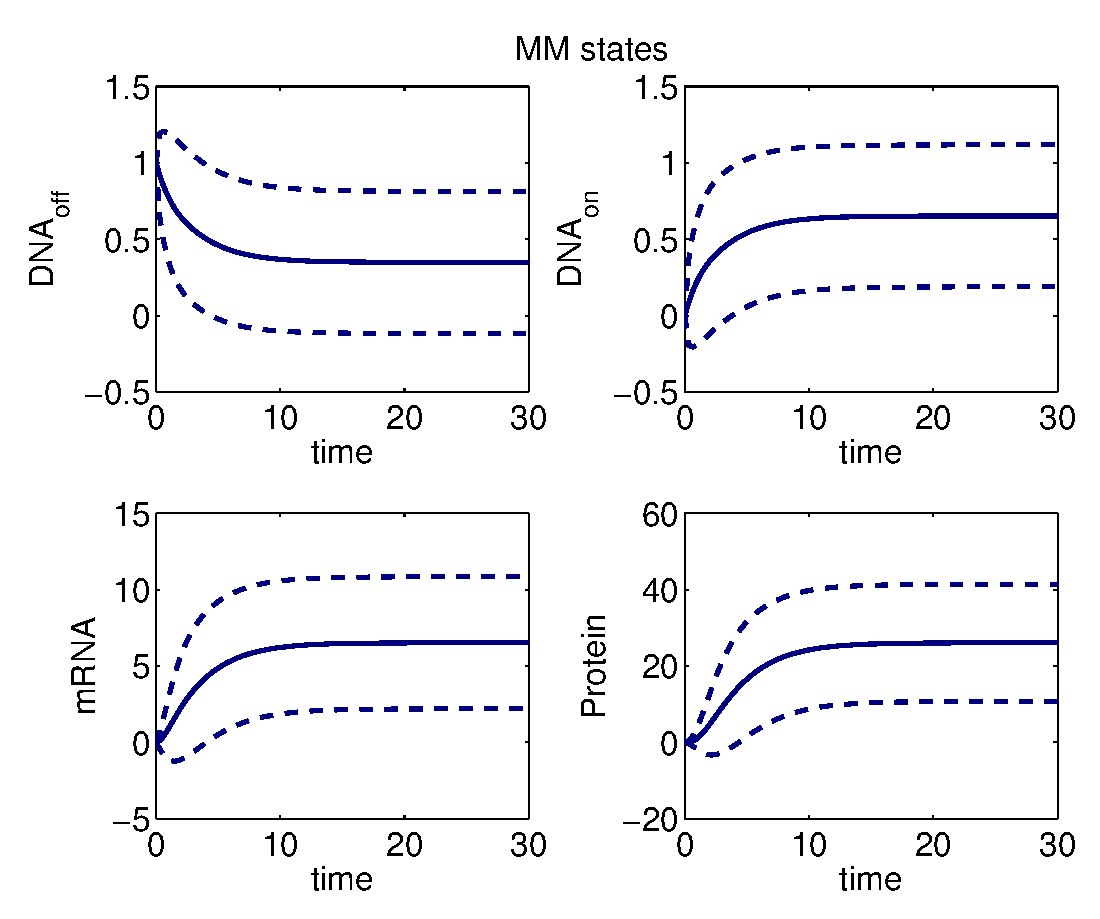
\includegraphics[scale=0.4]{figures1/MM_states}
\label{fig_MM_states}
}\subfigure[]{
\includegraphics[scale=0.4]{figures1/MM_outputs}
\label{fig_MM_outputs}
}
\caption{\ak{\textbf{Visualization of the \acrshort{mm} simulation results for \ex.}}
(a)~Mean of species including the 1-$\sigma$ intervals.
(b)~Mean of output variables including the 1-$\sigma$ intervals.
}
\label{fig_MM_vis}
\end{figure}

To plot the 2$^\text{nd}$ and 3$^\text{rd}$-order moments of the species (Figure~\ref{fig_MM_vis_ho}), the following options are set:
\begin{lstlisting}
options.plot_xo = 1;
options.state_order = 3;
plotMM(System_MM,options) 
\end{lstlisting}

\begin{figure}[t]
\centering
\subfigure[]{
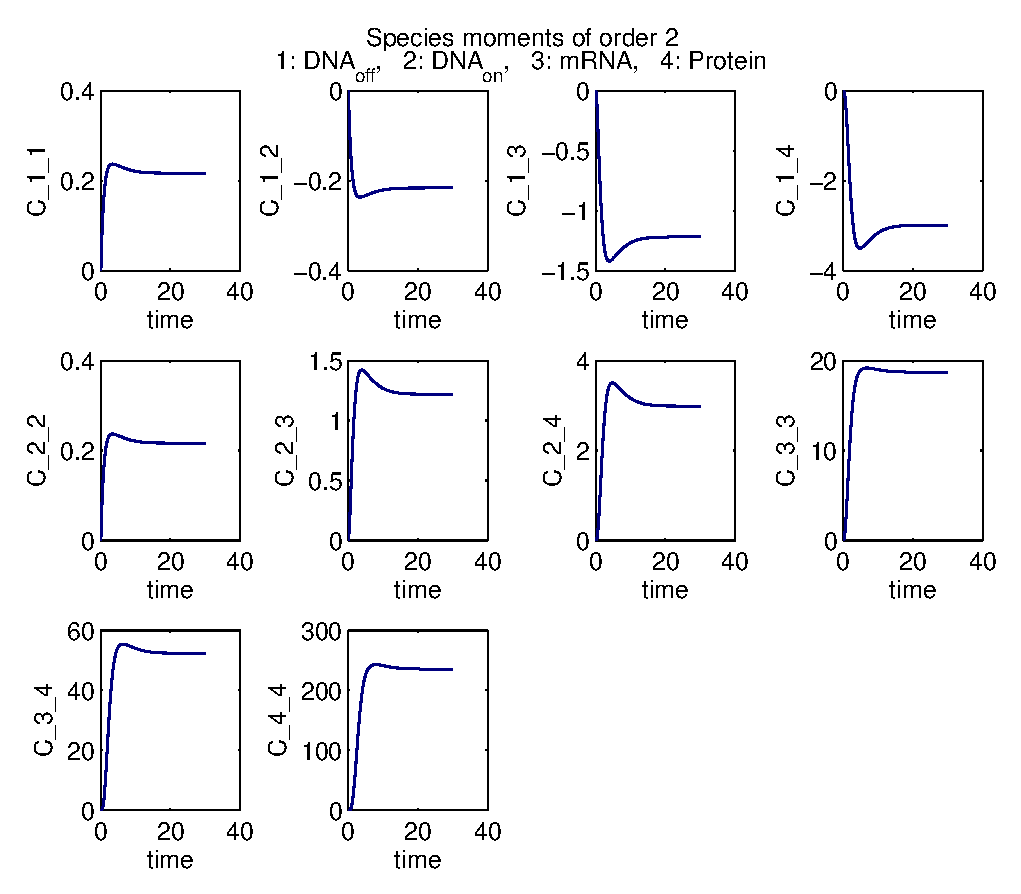
\includegraphics[scale=0.65]{figures1/Species_moments_of_order_2}
\label{fig_MM_states_o2}
}
\subfigure[]{
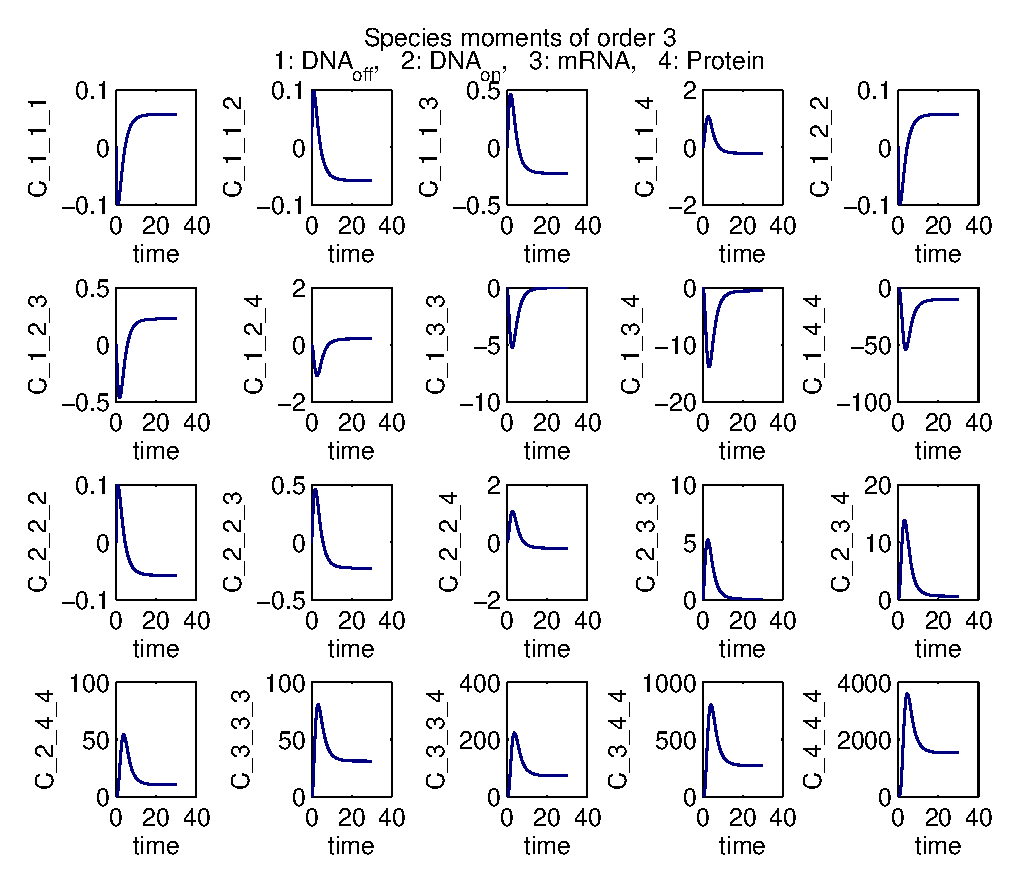
\includegraphics[scale=0.65]{figures1/Species_moments_of_order_3}
\label{fig_MM_states_o3}
}
\caption{\ak{\textbf{Visualization of higher-order moments in \exs using \acrshort{mm} simulation.}}
(a)~Second-order moments of species.
(b)~Third-order moments of species.
}
\label{fig_MM_vis_ho}
\end{figure}


Similarly, the states of the \acrshort{ios} simulation (see Section~\ref{ex_num_sim_sens}), together with the moments of species and the output moments, can be visualized as below (see Figure~\ref{fig_SSE_vis} and Figure~\ref{fig_SSE_vis_moments}):
\begin{lstlisting}
plotSSE(System_IOS) 
\end{lstlisting}

\begin{figure}[t]
\centering
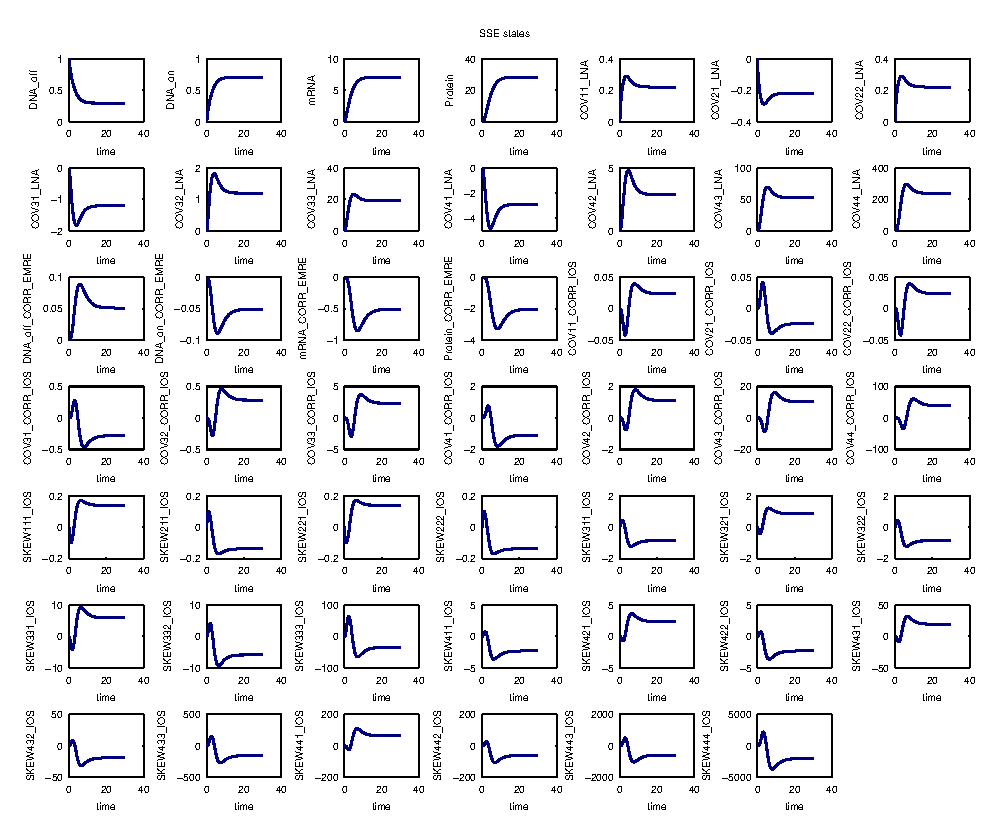
\includegraphics[scale=1]{figures1/SSE_states}
\caption{\ak{\textbf{Visualization of the \acrshort{sse} states for \ex.}}
}
\label{fig_SSE_vis}
\end{figure}

\begin{figure}[t]
\centering
\subfigure[]{
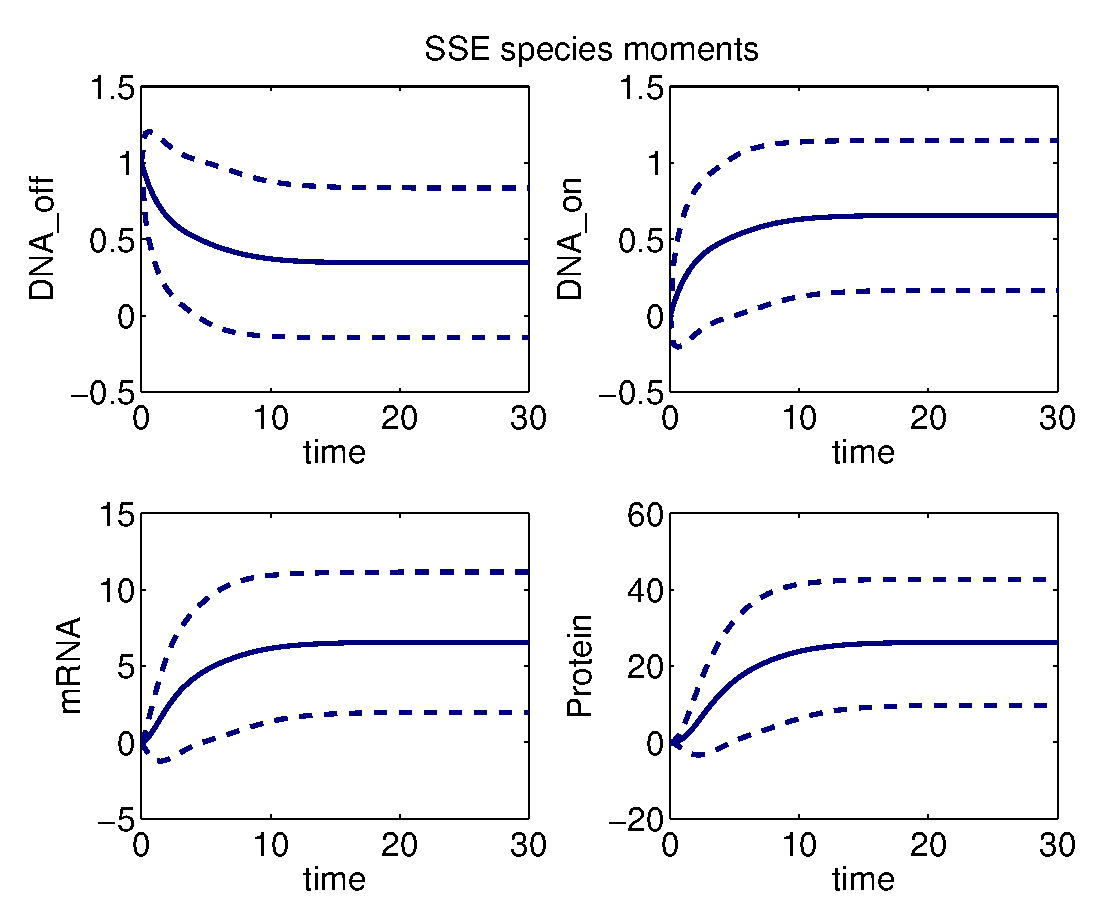
\includegraphics[scale=0.45]{figures1/SSE_species_moments}
\label{fig_SSE_species}
}\subfigure[]{
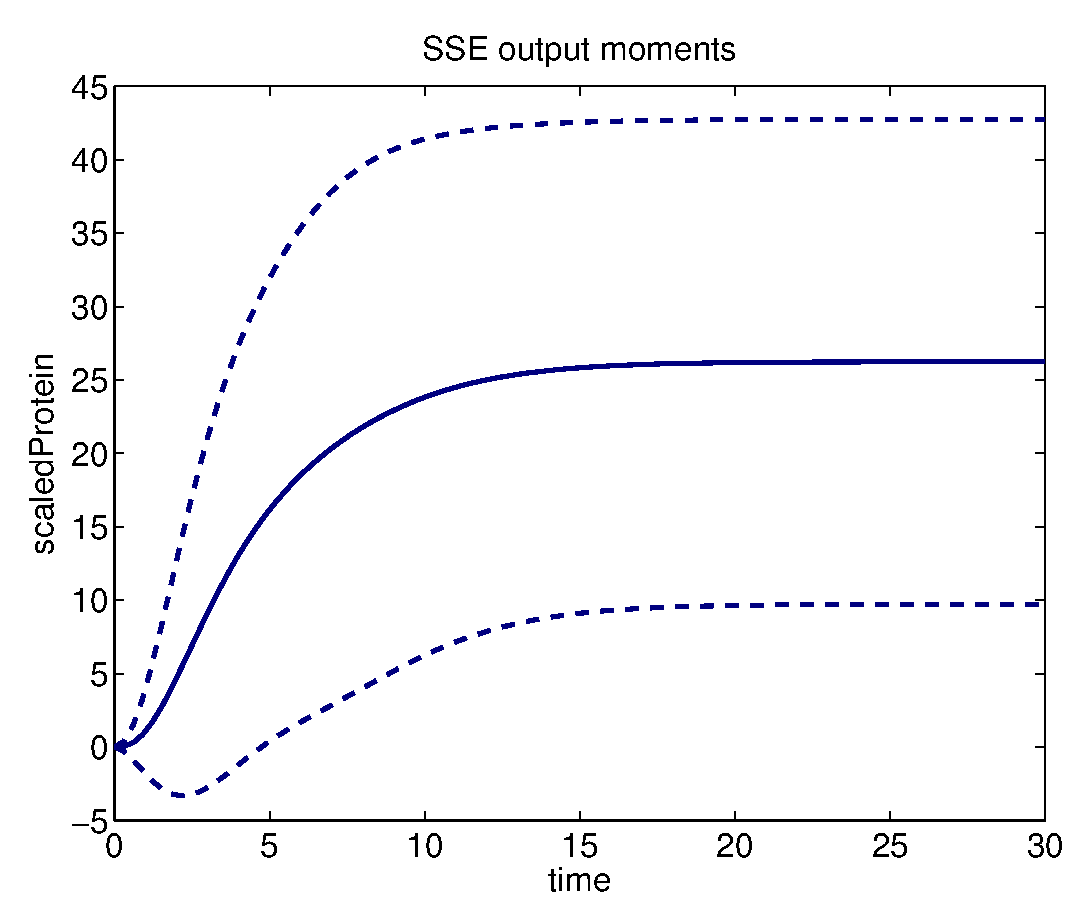
\includegraphics[scale=0.45]{figures1/SSE_output_moments}
\label{fig_SSE_outputs}
}
\caption{\ak{\textbf{Visualization of the moments of species and the output variables in \exs obtained by the \acrshort{sse} simulation.}}
(a)~Mean of species including the 1-$\sigma$ intervals.
(b)~Mean of output variables including the 1-$\sigma$ intervals.
}
\label{fig_SSE_vis_moments}
\end{figure}


%In addition, the moments of species can be plotted using the following (see Figure~\ref{fig_SSE_vis_moments}):
%\begin{lstlisting}
%options.species_moments = 1;
%plotSSE(System_IOS,options) 
%\end{lstlisting}

The results of \acrshort{mm}, \acrshort{mcm}, and \acrshort{ios} simulations are plotted together as below, and the resulting plots are shown in Figure~\ref{fig_compare}:
\begin{lstlisting}
SystemAll{1} = System_MM;
SystemAll{2} = System_MCM;
SystemAll{3} = System_IOS;
plotCompare(SystemAll)
\end{lstlisting}

\begin{figure}[t]
\centering
\subfigure{
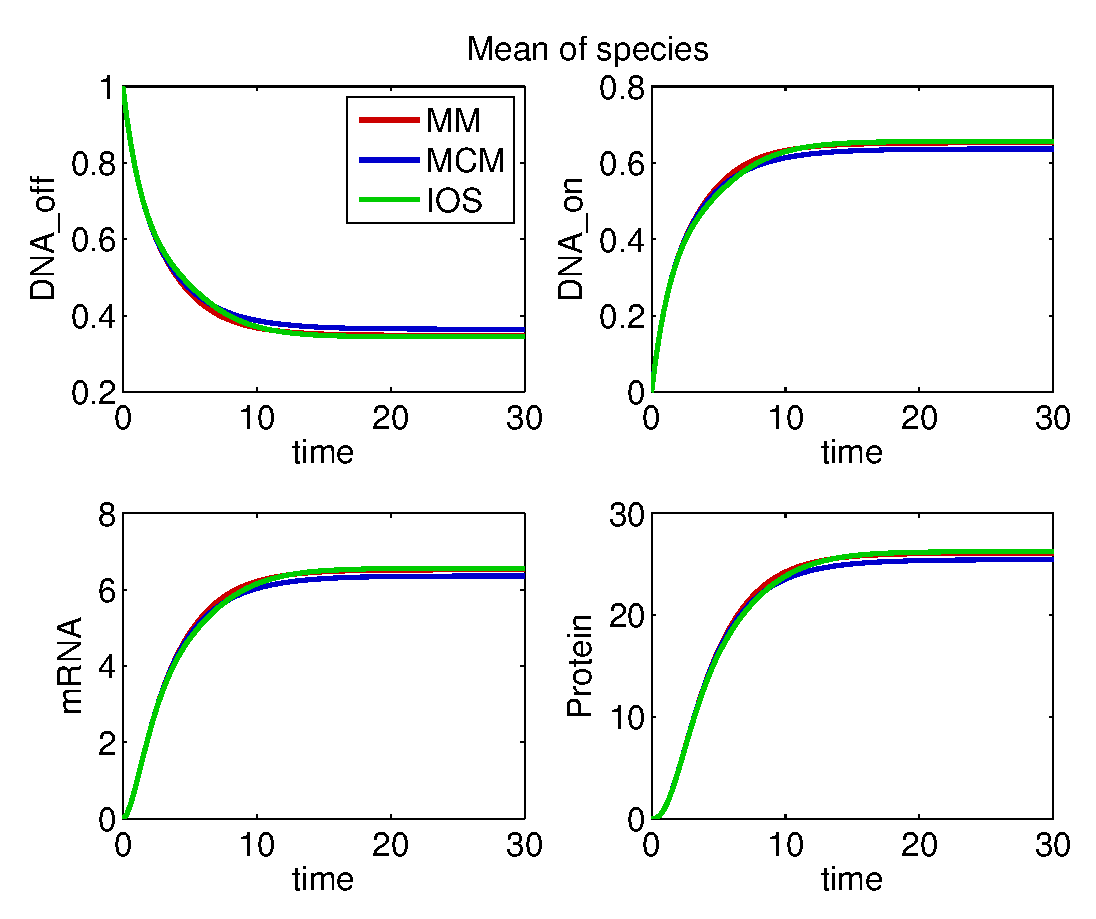
\includegraphics[scale=0.4]{figures1/Mean_of_species}
\label{fig_compare_mean_species}
}\subfigure{
\includegraphics[scale=0.4]{figures1/Variance_of_species}
\label{fig_compare_var_species}
}
\subfigure{
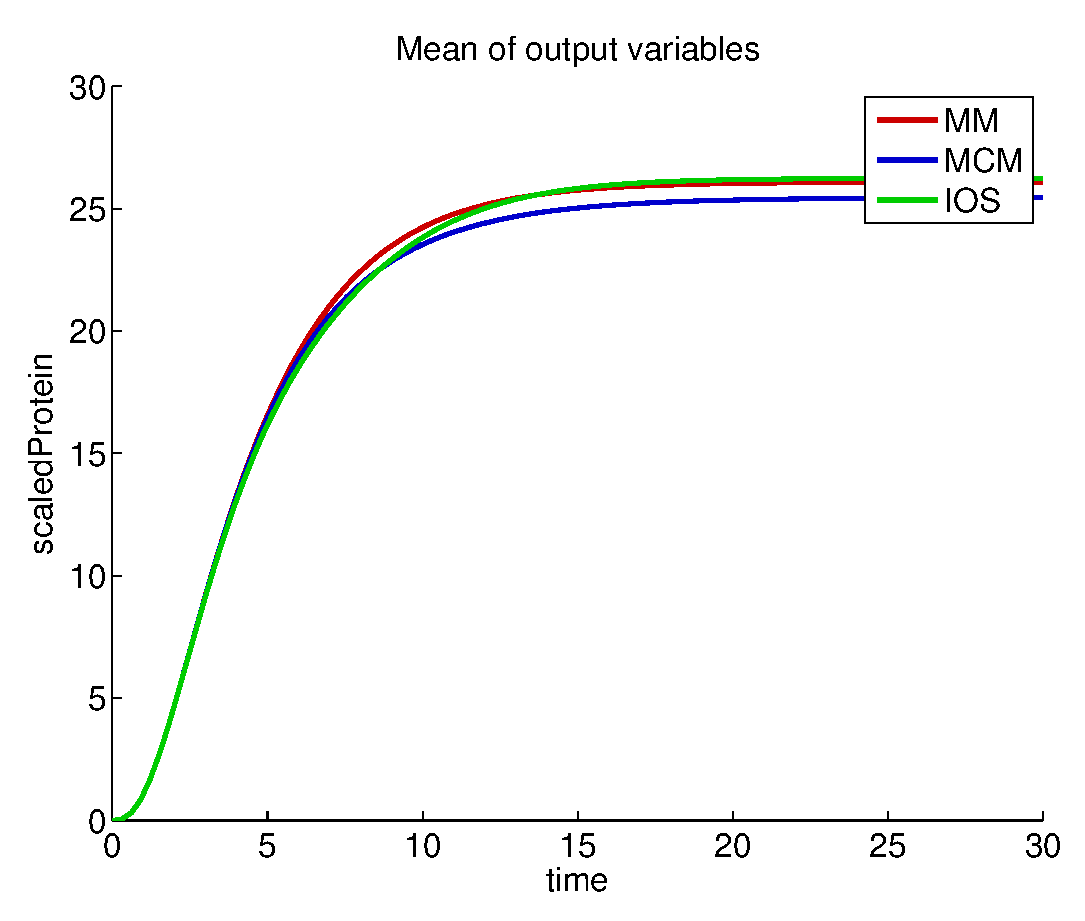
\includegraphics[scale=0.4]{figures1/Mean_of_output_variables}
\label{fig_compare_mean_outputs}
}\subfigure{
\includegraphics[scale=0.4]{figures1/Variance_of_output_variables}
\label{fig_compare_var_outputs}
}
\caption{\ak{\textbf{Mean and variance of species and output variables in \exs obtained by the \acrshort{mm}, the \acrshort{mcm} and the \acrshort{ios} simulations.}}
}
\label{fig_compare}
\end{figure}



\chapter{Further examples}
\section{JAK-STAT signaling pathway}
The second example studied using \toolboxnameSpace is a model of the JAK-STAT signaling pathway introduced by~\cite{Raue2009}.
The model, sketched in Figure~\ref{fig_ex2}, describes the signaling cascade of STAT protein.
Upon activation, Epo receptor triggers the phosphorylation of cytoplasmic STAT.
Dimerization and translocation of phosphorylated STAT into the nucleus, followed by a delayed export of STAT from the nucleus complete the loop.
The time-dependent concentration of phosphorylated Epo receptor, [pEpoR], functions as an input to the system.
%The experimental data for the concentration of phosphorylated Epo receptor, cytoplasmic STAT and phosphorylated cytoplasmic STAT are available from previous studies~\cite{Swameye2003}.

The JAK-STAT signaling pathway is an interesting application example as it (i) includes two compartments, namely cytoplasm and nucleus, and (ii) involves a time-dependent propensity.
Given the parameter values and initial conditions in Table~\ref{tab_ex2}, this pathway is simulated using several modeling approaches, including \acrshort{ssa}.

The \acrshort{ssa} simulation results, are plotted using the command below, and are shown in Figures~\ref{fig_jakstat_real}~and~\ref{fig_jakstat_mom}:
\begin{lstlisting}
options.fs = 10;
plotSSA(System_SSA,options)
\end{lstlisting}

The model definition and simulation files for this system can be found in \texttt{CERENA/examples/JakStat}.

\begin{figure}
\centering
\includegraphics[scale=0.75]{figures/ex2_3}
\caption{Schematic of the simplified JAK-STAT signaling pathway.}
\label{fig_ex2}
\end{figure}
\begin{table}
\caption{Parameter values and initial conditions of \ex.}
\centering
\begin{tabular}{|c|c|}
\hline
$p_1$ & 3.9364\\ \hline
$p_2$ & 10\\ \hline
$p_3$ & 0.1125\\ \hline
$p_4$ &0.9829\\ \hline
$X_{c,\text{STAT}}(0)$ & 1\\ \hline
$X_{c,\text{pSTAT}}(0)$ & 0\\ \hline
$X_{c,\text{pSTAT-pSTAT}}(0)$ & 0\\ \hline
$X_{c,\text{npSTAT-npSTAT}}(0)$ & 0\\ \hline
$X_{c,\text{npSTAT1}}(0)$ & 0\\ \hline
 $X_{c,\text{npSTAT2}}(0)$ & 0\\ \hline
 $X_{c,\text{npSTAT3}}(0)$& 0\\ \hline
 $X_{c,\text{npSTAT4}}(0)$& 0\\ \hline
 $X_{c,\text{npSTAT5}}(0)$ & 0\\ \hline
\end{tabular}
\label{tab_ex2}
\end{table}
\begin{figure}
\centering
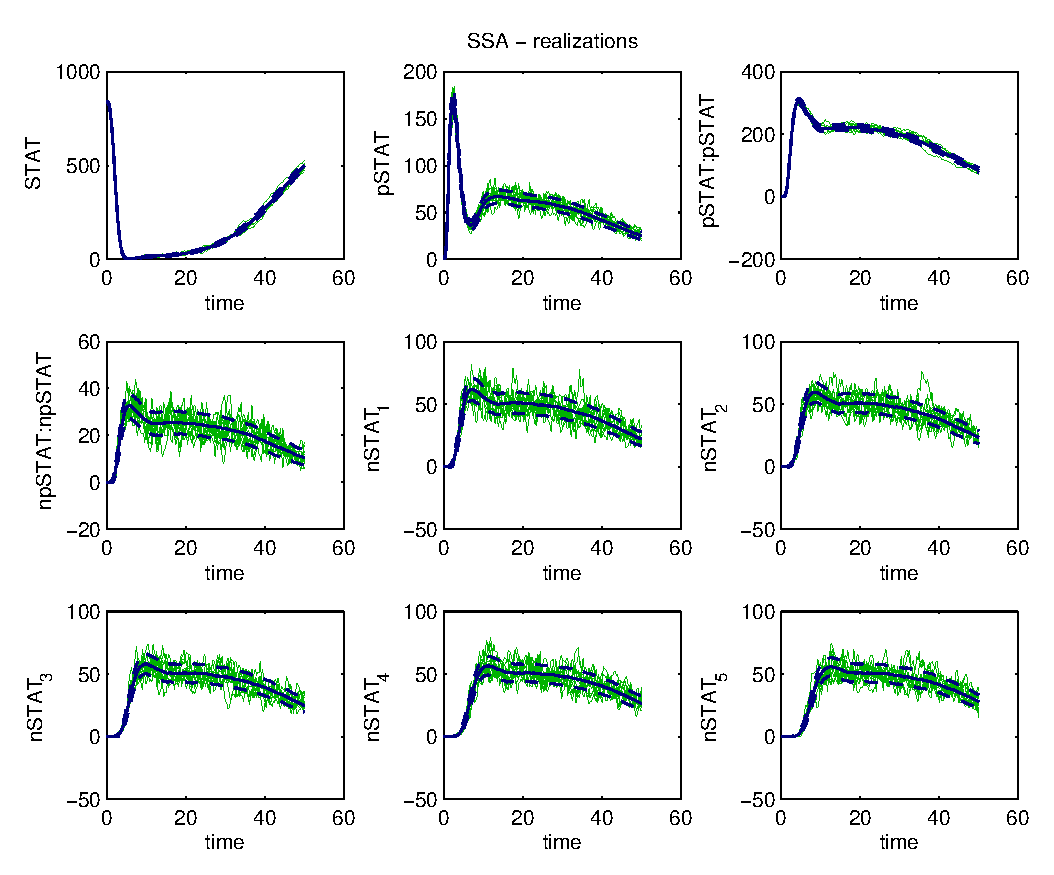
\includegraphics[scale=0.75]{figures1/SSA-realizations}
\caption{\textbf{\acrshort{ssa} simulation results for the simplified JAK-STAT pathway.} Individual realizations (green) and the mean of the counts of species including 1-$\sigma$ intervals (blue) are shown.}
\label{fig_jakstat_real}
\end{figure}
\begin{figure}
\centering
\subfigure{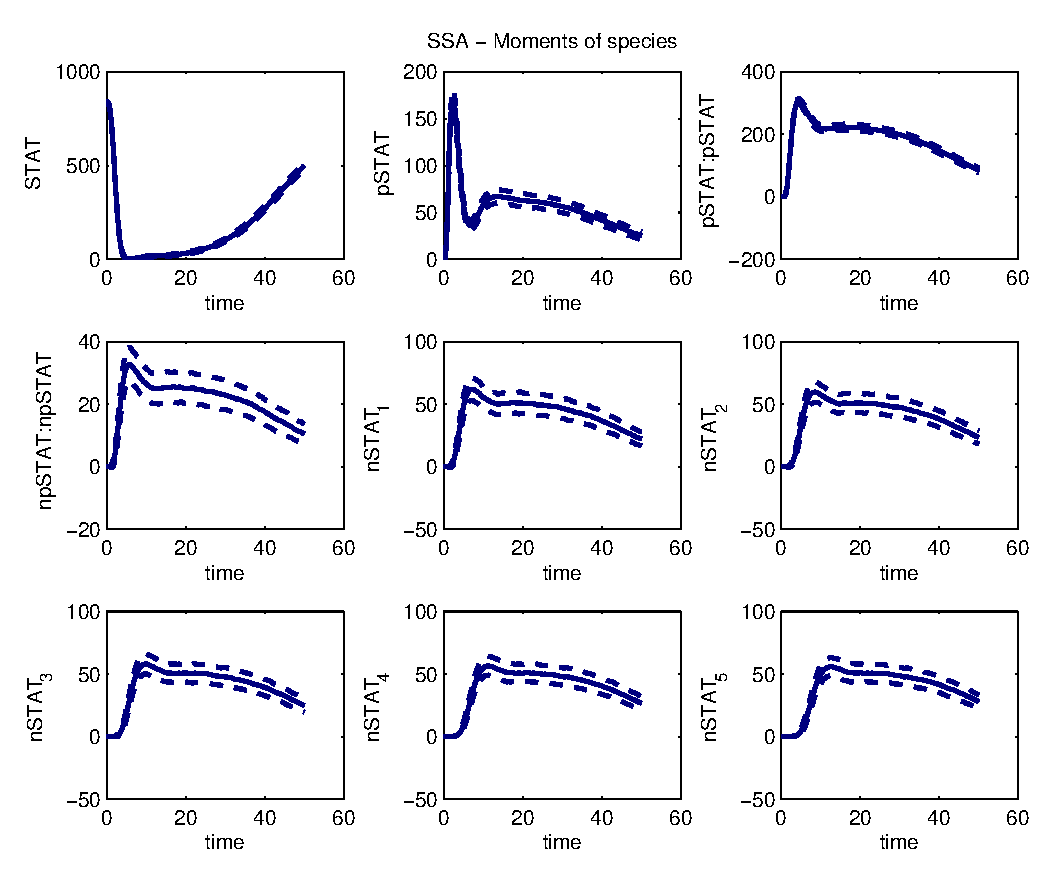
\includegraphics[scale=0.5]{figures1/SSA-Moments-of-species}
\label{fig_jakstat_mom_x}
}\subfigure{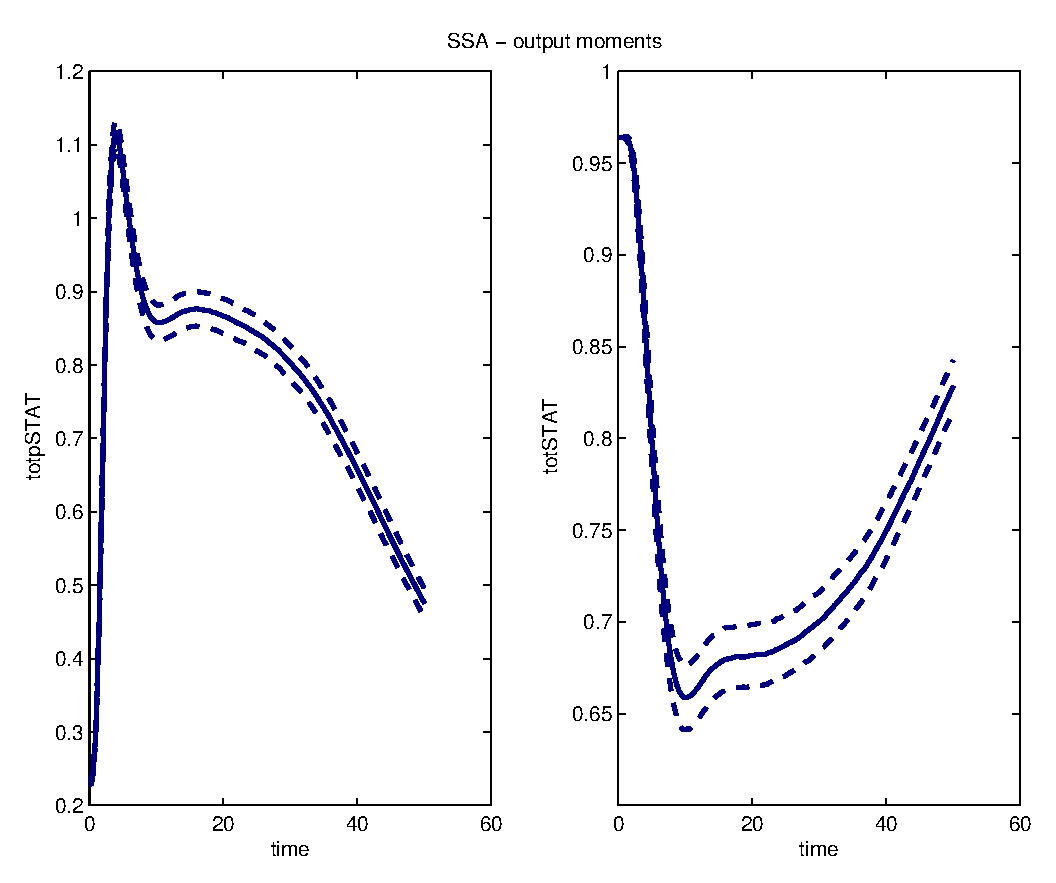
\includegraphics[scale=0.5]{figures1/SSA-output-moments}
\label{fig_jakstat_mom_y}}
\caption{\textbf{The counts of species and the concentration of the observable, i.e. total concentration of STAT, obtained by \acrshort{ssa} simulation.} The means, including 1-$\sigma$ intervals, are shown.}
\label{fig_jakstat_mom}
\end{figure}

\newpage
\section{PapI regulation model}
This model, sketched in Figure~\ref{fig_papi}, describes the regulation of Pap pili formation on the surface of \emph{E.~coli}~\cite{KazeroonianThe2014}. 
This system includes a a \emph{pap} operon and regulatory proteins LRP and PapI.
Binding of LRP to either or both of the binding sites results in four configurations of the \emph{pap} operon.
Only if the operon is in state $\text{g}_2$, pili can be produced.
PapI sets up a a positive feedback loop for the production of pili by reducing the unbinding rate of LRP from the operon.

This process is an interesting application example as it involves non-polynomial propensity functions. 
The model definition and simulation files for this system can be found in \texttt{CERENA/examples/PapI}.

\begin{figure}
\centering
\includegraphics[scale=0.3]{figures/papi_model}
\caption{\textbf{Schematic of the PapI regulation model.} Arrows represent the binding and unbinding of LRP to/from the operon. Dotted arrows indicate the influence of PapI on the reaction rates. }
\label{fig_papi}
\end{figure}

\section{A gene cascade network}
A gene cascade network, described in~\cite{SinghHes2011}, is implemented in \toolboxname.
The model definition and simulation files can be looked up in \texttt{CERENA/examples/geneCascade}.

%\gls{def_file}.
%
%\acrshort{mm}, \acrlong{mm}
%\normalsize
%\bibliographystyle{natbib}
%\newcommand{\bibfont}{\normalfont\footnotesize}
% Use the PLoS provided BiBTeX style
\bibliographystyle{plos2015}
%\bibliography{Database_jh}
\begin{thebibliography}{10}

\bibitem{ShahrezaeiSwa2008}
Shahrezaei V, Swain PS.
\newblock Analytical distributions for stochastic gene expression.
\newblock {Proc Natl Acad Sci USA}. 2008 Nov;105(45):17256--17261.

\bibitem{Norris1997}
Norris JR.
\newblock Continuous-time Markov chains I.
\newblock In: Markov Chains. Cambridge University Press; 1997. p. 60--107.
\newblock Cambridge Books Online.
%\newblock Available from: \url{http://dx.doi.org/10.1017/CBO9780511810633.004}.

\bibitem{Gillespie1977}
Gillespie DT.
\newblock Exact stochastic simulation of coupled chemical reactions.
\newblock J Phys Chem. 1977 Dec;81(25):2340--2361.

\bibitem{Anderson2007}
Anderson DF.
\newblock A modified next reaction method for simulating chemical systems with
  time dependent propensities and delays.
\newblock J Chem Phys. 2007 Dec;127(214107).

\bibitem{MunskyKha2006}
Munsky B, Khammash M.
\newblock The finite state projection algorithm for the solution of the
  chemical master equation.
\newblock J Chem Phys. 2006 Jan;124(4):044104.

\bibitem{vanKampen2007}
{van Kampen} NG.
\newblock Stochastic processes in physics and chemistry.
\newblock 3rd ed. Amsterdam: North-Holland; 2007.

\bibitem{Grima2010}
Grima R.
\newblock An effective rate equation approach to reaction kinetics in small
  volumes: Theory and application to biochemical reactions in nonequilibrium
  steady-state conditions.
\newblock J Chem Phys. 2010 July;133(035101).

\bibitem{ThomasMat2013}
Thomas P, Matuschek H, Grima R.
\newblock How reliable is the linear noise approximation of gene regulatory
  networks?
\newblock BMC Genomics. 2013 Oct;14(Suppl 4)(S5).

\bibitem{RamaswamyGon2012}
Ramaswamy R, Gonz\'alez-Segredo N, Sbalzarini I, Grima R.
\newblock Discreteness-induced concentration inversion in mesoscopic chemical
  systems.
\newblock Nat Comm. 2012 Apr;3(779).

\bibitem{Engblom2006}
Engblom S.
\newblock Computing the moments of high dimensional solutions of the master
  equation.
\newblock Appl Math Comp. 2006;180:498--515.

\bibitem{LeeKim2009}
Lee CH, Kim KH, Kim P.
\newblock A moment closure method for stochastic reaction networks.
\newblock J Chem Phys. 2009 Apr;130(13):134107.

\bibitem{SinghHes2011}
Singh A, Hespanha JP.
\newblock Approximate moment dynamics for chemically reacting systems.
\newblock {IEEE} Trans Autom Control. 2011 Feb;56(2):414--418.

\bibitem{HasenauerWol2014}
Hasenauer J, Wolf V, Kazeroonian A, Theis FJ.
\newblock Method of conditional moments ({MCM}) for the chemical master
  equation.
\newblock J Math Biol. 2014 Aug;69(3):687--735.

\bibitem{RaueSch2013}
Raue A, Schilling M, Bachmann J, Matteson A, Schelke M, Kaschek D, et~al.
\newblock Lessons learned from quantitative dynamical modeling in systems
  biology.
\newblock {PL}o{S} {ONE}. 2013 Sept;8(9):e74335.

\bibitem{HindmarshBro2005}
Hindmarsh AC, Brown PN, Grant KE, Lee SL, Serban R, Shumaker DE, et~al.
\newblock {SUNDIALS:} {S}uite of {N}onlinear and {D}ifferential/{A}lgebraic
  {E}quation {S}olvers.
\newblock ACM T Math Software. 2005 Sept;31(3):363--396.

\bibitem{Keating2006}
Keating SM, Bornstein BJ, Finney A, Hucka M.
\newblock SBMLToolbox: an SBML toolbox for MATLAB users.
\newblock Bioinformatics. 2006;22(10):1275--1277.
\newblock Available from:
  \url{http://bioinformatics.oxfordjournals.org/content/22/10/1275.abstract}.

\bibitem{RaueSte2015}
Raue A, Steiert B, Schelker M, Kreutz C, Maiwald T, Hass H, et~al.
\newblock Data2Dynamics: a modeling environment tailored to parameter
  estimation in dynamical systems.
\newblock Bioinformatics. 2015 Jul.

\bibitem{Schafer2005}
Schafer J, Strimmer K.
\newblock A shrinkage approach to large-scale covariance matrix estimation and
  implications for functional genomics.
\newblock Stat Appl Genet Mol Biol. 2005;4:Article32.

\bibitem{OpgenRhein2007}
Opgen-Rhein R, Strimmer K.
\newblock Accurate ranking of differentially expressed genes by a
  distribution-free shrinkage approach.
\newblock Stat Appl Genet Mol Biol. 2007;6:Article9.

\bibitem{Raue2009}
Raue A, Kreutz C, Maiwald T, Bachmann J, Schilling M, Klingm\"uller U, et~al.
\newblock Structural and practical identifiability analysis of partially
  observed dynamical models by exploiting the profile likelihood.
\newblock Bioinf. 2009 May;25(25):1923--1929.

\bibitem{KazeroonianThe2014}
Kazeroonian A, Theis FJ, Hasenauer J.
\newblock Modeling of stochastic biological processes with non-polynomial
  propensities using non-central conditional moment equation.
\newblock In: Proc. of the 19th {IFAC} World Congress. vol.~19. Cape Town,
  South Africa; 2014. p. 1729--1735.

\end{thebibliography}

\clearpage
\printglossary[type=\acronymtype]
\printglossary
\end{document}  